%FIX tables 6 different apps   

% REMEMBER: You must not plagiarise anything in your report. Be extremely careful.

\documentclass{l4proj}

%FIX refer to figures

    
%
% put any additional packages here
%

\begin{document}

%==============================================================================
%% METADATA
\title{Level 4 Project Report Template}
\author{John H. Williamson}
\date{September 14, 2018}

\maketitle

%==============================================================================
%% ABSTRACT
\begin{abstract}
    Every abstract follows a similar pattern. Motivate; set aims; describe work; explain results.
    \vskip 0.5em
    ``XYZ is bad. This project investigated ABC to determine if it was better. 
    ABC used XXX and YYY to implement ZZZ. This is particularly interesting as XXX and YYY have
    never been used together. It was found that  
    ABC was 20\% better than XYZ, though it caused rabies in half of subjects.''
\end{abstract}

%==============================================================================

% EDUCATION REUSE CONSENT FORM
% If you consent to your project being shown to future students for educational purposes
% then insert your name and the date below to  sign the education use form that appears in the front of the document. 
% You must explicitly give consent if you wish to do so.
% If you sign, your project may be included in the Hall of Fame if it scores particularly highly.
%
% Please note that you are under no obligation to sign 
% this declaration, but doing so would help future students.
%
%\def\consentname {My Name} % your full name
%\def\consentdate {20 March 2018} % the date you agree
%
\educationalconsent


%==============================================================================
\tableofcontents

%==============================================================================
%% Notes on formatting
%==============================================================================
% The first page, abstract and table of contents are numbered using Roman numerals and are not
% included in the page count. 
%
% From now on pages are numbered
% using Arabic numerals. Therefore, immediately after the first call to \chapter we need the call
% \pagenumbering{arabic} and this should be called once only in the document. 
%
% Do not alter the bibliography style.
%
% The first Chapter should then be on page 1. You are allowed 40 pages for a 40 credit project and 30 pages for a 
% 20 credit report. This includes everything numbered in Arabic numerals (excluding front matter) up
% to but excluding the appendices and bibliography.
%
% You must not alter text size (it is currently 10pt) or alter margins or spacing.
%
%
%==================================================================================================================================
%
% IMPORTANT
% The chapter headings here are **suggestions**. You don't have to follow this model if
% it doesn't fit your project. Every project should have an introduction and conclusion,
% however. 
%
%==================================================================================================================================
\chapter{Introduction}

% reset page numbering. Don't remove this!
\pagenumbering{arabic} 



Why should the reader care about what are you doing and what are you actually doing?
\section{Guidance}

\textbf{Motivate} 
Activity trackers are very popular nowadays. These apps leverage various motivators, such as social feeds, points for activity, and reminders. However, most of these apps do not leverage collaborative motivators. I wanted to investigate whether or not users would feel more motivated to exercise if it wasn't just about working towards a personal goal, but towards a shared goal with a team of friends/strangers. The goal of my RPG themed activity tracker, 'Stat Buff' was to gamify progress as ingame character development (leading to greater attack damage), and workouts as attacks towards your teams enemy. This rewards users for making progress in their performance, as well as for making small daily efforts. The teams enemy resets in a week if it has not been defeated, which creates an urgency to exercise in order to to reach the next enemy.
\section{Writing guidance}
\subsection{Who is the reader?}

This is the key question for any writing. Your reader:

Remember, you will be marked by your supervisor and one or more members
of staff. You might also have your project read by a prize-awarding
committee or possibly a future employer. Bear that in mind.

\subsection{References and style guides}

\subsubsection{Citation styles}

%\item If you are referring to a reference as a noun, then cite it as: ``\citet{Orw68} discusses the role of language in political thought.''
%\item If you are referring implicitly to references, use: ``There are many good books on writing \citep{Orw68, Wil09, Pin15}.''

There is a complete guide on good citation practice by Peter Coxhead available here: \url{http://www.cs.bham.ac.uk/~pxc/refs/index.html}. 
If you are unsure about how to cite online sources, please see this guide: \url{https://student.unsw.edu.au/how-do-i-cite-electronic-sources}.

\subsection{Plagiarism warning}

\begin{highlight_title}{WARNING}
    
    If you include material from other sources without full and correct attribution, you are commiting plagiarism. The penalties for plagiarism are severe.
    Quote any included text and cite it correctly. Cite all images, figures, etc. clearly in the caption of the figure.
\end{highlight_title}


%==================================================================================================================================
\chapter{Background}
 
%FIX
%https://dl.acm.org/doi/10.1145/2592235.2592240
%https://dl.acm.org/doi/10.1145/1125451.1125805
%https://dl.acm.org/doi/10.1007/11853565_16
%https://link.springer.com/article/10.1007/s11036-007-0011-7
%https://dl.acm.org/doi/10.1145/3134717

%start of the background, roadmap the issues, lot of them involved with step counts 
% 
I started my research by analyzing existing collaborative exercise apps. I only found one research paper on this topic. This paper was on "Pass the Ball" an app which was developed in order to evaluate the effectiveness of enforced turn taking for encouraging exercise \citep{Pass_the_ball}. In the second version of the app, users in groups had a single ball which gave the owner the ability to score points for the team through exercise, which could be passed to other users. Users who received the ball often felt that they had a small window of opportunity to score points before someone else wanted the ball. For example, one participant said: "I turned to my group and I was like 'we’re walking fast today! We have an hour to get as many steps in as we can!'". This exclusivity also caused some issues. Users who stole the ball from another teammate (incuring a penalty) would get into fights with other members. One user sent the message "Sorry, Just looked at my phone. I would have passed!" after their ball was stolen. Although the app seemed to make some group members competitive and more passionate about exercise, there were some drawbacks to their implementation "such as obligation, conflict, and privacy concerns".

I wanted to make the game RPG themed, so I looked into if there were any RPG themed activity trackers. I found a study on a game called Spyfeet \citep{SpyFeet}. SpyFeet is a pedometer combined with story-telling elements. The more the user walks, the more they progress in the story. Although this was a singleplayer game and much more story-driven than what I wanted to make, it was reassuring to see that additional reward for exercise leads to more activity.

I then continued my research by looking into analysis of the state of top activity trackers. The paper by \citet{Behavior_change} discusses the lack of behavioural change techniques employed in top activity trackers. The researchers divided activity trackers into two categories: educational and motivational. This is an important consideration, as they proposed education and motivation as a continuum, where emphasis of one diminishes the other. This was an important consideration, as I realized that I would not be able to simultaneously target the app towards those who do not know how to exercise, and motivational for users who already know how to train.

\citet{AppsOfSteel} performed the same analysis as the afformentioned paper, but evaluated the apps more quantitatively. They scored each app out of 100 based on the presence behavioural change techniques or absence of bad practices. The average top app scored 11/100, some as low as 1/100, with the best app scoring 28/100. These results signify that either users don't care whether their activity trackers include behavioural change techniques, or that users simply don't have a lot of good options.

I read \citet{User_expectations} as I wanted to better understand what users wanted from activity trackers, as I needed my app to contain enticing features in addition to the collaborative aspects. The app found that content was most important for 47.2\%, technical implementation and utilities 39.7\%, and psychological features were the most important for 13.2\% of users. This made me prioritize content and the technical implementation, as this would hopefully help maintain users.

I was curious if it was possible to implement reinforcement learning in order to vary behavioural change techniques to accomodate for a wide array of users. I found a paper on the topic \citet{Personalizing}, but this only varied step count based on the steps that users were taking. The research found that users provided with dynamic goals exercised more than the control group which performed no exercise. This could have been an interesting addition to my app, but it was out of scope for me to implement.

Finally, I did some research into behavioural change techniques in general. There were lots of categories of behaviour change, one of which was social support/accountability. Most of the techniques were not feasible to implement, but understanding the importance of social support and accountability and how it can be implemented was helpful for my own implementation. \citep{Integrated_Theory}

I analyzed existing exercise apps, and existing RPG games in order to better understand the two categories I am combining. I analyzed Stronglifts 5x5 and Jefit, two popular exercise apps. Both had inbuilt social features, and online forums to keep people motivated. They had some complicated exercise features like planning workouts, which were out of scope for me. I found that Jefit had competitions, but no collaborative exercising. The absence of collaborative features showed that there was room to explore the effectiveness of these apps. I had to make sure that I implemented at least some of the features of existing popular exercise apps in order to maintain user engagement. These were the key features that I noticed in both these apps:

%FIX add screenshots 
%add table containing characteristics 
\begin{itemize}    
    \item
      Social features (adding friends/chatting)
    \item
      Being able to plan workouts
    \item
      Being able to track a wide variety of exercises
    \item 
      Built in exercise tutorials
    \item
      Satisfying animations/congratulating progress
    \item
      Progression suggestions (add more or less weight)
\end{itemize}

From my analysis of RPG games, I realized that collaboration is an integral part of RPG games, and that existing products should serve as a model for implementing collaborative aspects. For instance, Clash of Clans has clans, where users need to give each other troops in order to defend one another. Clans also battle against one another in "Clan Wars" where users have to attack each others bases in order to win. Wins require members to attack consistently and to reinforce their fellow members \citep{coc}. 
Another example of a collaborative RPG is World of Warcraft. In World of Warcraft, users participate in Raids together, which require very detailed coordination from all members. There are also multiple different roles which users have to take, such as healer, tank, or DPS (damage dealer) \citep{wow}. There is a viral video where a World of Warcraft player named "Leeroy Jenkins" ruins an entire raid by going in alone as the team plans their attack, ruining their whole raid \citep{leeroy_jenkins}. Even many singleplayer RPG games are built around collaboration. For instance the game Darkest Dungeon \citet{darkest_dungeon} is built around controlling your various heroes, who can give each other status bonuses, and heal each other. For instance, the Plague Doctor hero is focused on healing others, while a Highwayman can deal lots of damage. From these three RPG collaborative games, I derived the following key points:

\begin{itemize}    
    \item
      Teams should fight against other players (or non-player characters)
    \item
      Users should be encouraged to help each other
    \item
      Users should have specific roles that serve some purpose in achieving the end goal.
    \item 
      There should be some clear progression: both on an individual level and on a team level. These should be linked (the team should progress faster if individual users are progressing)
    \item 
      There should be accountability: if some user(s) aren't doing their part, they should not progress.
\end{itemize}



\section{Guidance}
\begin{itemize}    
    \item
      Don't give a laundry list of references.
    \item
      Tie everything you say to your problem.
    \item
      Present an argument.
    \item Think critically; weigh up the contribution of the background and put it in context.    
    \item
      \textbf{Don't write a tutorial}; provide background and cite
      references for further information.
\end{itemize}

%==================================================================================================================================
\chapter{Analysis/Requirements}
%FIX add citations 
Exercise is hard to do consistently, leading to high inactivity. Social and group based exercise (such as exercising with a friend or joining a class) are good solution for making people feel accountable, and forcing a schedule. Even then, exercise would still be for your own good, and not for some common goal. A collaborative activity tracker would try to remove the buy in of group based exercise (course cost, fixed schedule) and would make the user feel as though they were contributing to a collective success and not just an individual one. 
\section{Guidance}
Make it clear how you derived the constrained form of your problem via a clear and logical process. 

%==================================================================================================================================
\chapter{Design}

A key feature of collaborative activity trackers is that exercise must have some collective benefit beyond just the individual benefit. I decided not to implement the turn-taking design of pass the ball, as it seemed to sometimes cause conflict and seemed difficult to implement well. Instead of users having to take turns, users could attack a monster enemy at any time through exercise. I liked the window of opportunity created from receiving the ball, so I added a maximum time to defeat the enemy before it resets. This should hopefully make users feel that their exercise is causing them to turn the tide of the battle, especially when they deal a killing blow on an enemy that is close to resetting.

\subsection{Calculating a user's contribution}
I wanted this app to calculate your team's contribution based on your effort and your strength. Rewarding effort should hopefully motivate users to workout regularly and push themselves, even when progress plateaus. Progress is rarely linear: it often has bumps, but through perseverance, you progress more than you regress. This also motivates users with lots of experience, as they can often feel demotivated by the waning progress, and the amount of time and effort it can take to accomplish something a beginner can achieve in a fraction of the time. I also reward strength, as I want the app to provide users with long term motivation. I don't want users to simply exercise for the sake of exercise, but also for the long-term improvements in strength. Rewarding progression is also important as it disincentivizes overtraining. If I only reward effort, the optimal strategy would be to exercise as much as possible, even if you felt pain or your progression stopped and regressed. By rewarding strength improvements, I reward the user for training moderately and resting adequately, as these are integral for long term progress. I gamify strength as attack damage, and effort as the number of attacks you deliver towards your team's enemy. The product of the two is the total damage that you deal towards your team's enemy. This total damage is dealt towards the monster that your enemy is currently fighting, and represents a members contribution to the group.

Initially I had to quantify strength, or attack damage. I wanted strength to be calculated relative to the person performing it. For example, it is harder for an average 50kg person to lift a certain weight, than for the average 80kg person. By taking this into account, I made the app more inclusive, and allowed everyone to contribute based on how strong they are relative to others like them, and not everyone else. Relative strength is simply a percentile that is calculated based on the demographic of the person, the exercise they performed, and the weight and repetitions that they used. There are sites which perform this calculation, which I will go into more detail in the implementation section. I was still left with the challenge of converting per-exercise percentiles into a single strength value. Initially, I used a simple naive implementation, where I took the mean percentile of all exercises, and used that as the final strength value. This is problematic, as this would encourage users to only track their best exercise, and nothing else. I don't want my app to encourage users to just focus on one exercise, as this can lead to injuries and imbalances. With this in mind, I decided that users should be rewarded for adding more exercises up to a certain number by setting strength to be the product of the average strength and the total number of tracked exercises. This seemed good, but this simplified to be just the sum of percentiles.

\begin{algorithm}[H]
  $\frac{\sum_{i=0}^{n} x_i}{n} * n = {\sum_{i=0}^{n} x_i}$
\end{algorithm}

I only realized this on the first day of the evalution. Luckily, this was a simple database function, so it was easy to replace this calculation. My final solution was to multiply the average strength percentage with the number of exercises log scaled, which only rewards adding more exercises up to a certain point. I think it's important to disincentivize laborious strategies such as keeping track of 50 exercises just because it would increase your total damage. 

\begin{algorithm}
  $attack\_damage = \frac{\sum_{i=1}^{n} x_i}{n} * ln(n) $

  where the user has tracked $n$ exercises, and $x$ contains the strength percentiles for exercises 
\end{algorithm}

Next, I had to decide how I would grant attacks based on workout effort. I could compare the user's per exercise performance relative to the last time. This would have a lot of confounding factors: personal differences and skill level let some add more weight with less effort. There would also be the problem of missing data (what is the effort on your first workout, or when you use new exercises?). This would also require users to input the number of repetitions and lifted weight for all their sets for all their exercises. Finally, this wouldn't reward users for putting in effort even on a bad day or during a plateau. I consulted sport science literature, and found a popular metric for estimating effort is called "RPE" (Rate of Perceived Exertion). RPE is a scale from 1-10, where 1 is almost no effort, 5 is moderate effort, and 10 is maximal effort. RPE has the downside of not being objective, as we are relying on a person's subjective perception of their effort. Research by Monica et al. found that "The odds of underestimating RPE for an exerciser were 3.67 times greater than a non-exerciser" \cite{RPE_estimations}. This could be offset by reducing the RPE that beginner's estimate, but this was out of scope for this project. I am not particularly worried about intentional dishonesty with regards to RPE, as users can lie about the number of sets they complete, how much they can lift, how often they train, etc. I decided to use RIR (repetitions in reserve), which is an inverse of RPE as it seemed easier to understand than RPE. This article \cite{rir} made a good case for measuring total training stress through average RIR and total sets. I couldn't find any specific equations that combined the two, so I created this equation, which increases as average RIR decreases and total sets increase.

\begin{algorithm}
  $granted\_attacks = min(0, (10 - average\_rir) * total\_sets)$
\end{algorithm}

With both attack\_damage, we can the damage dealt as 

\begin{algorithm}
  $workout\_damage = attack\_damage * granted\_attacks$ 
\end{algorithm}


\subsection{Communicating app functionality to the user}
When you open the app, you initially see two buttons on the top. One is labeled as "Strengthen Character" while the other one is labeled as "Deal Damage". "Strengthen Character" lets you update your exercise personal records, which increase your character's strength. "Deal Damage" on the other hand lets you track a workout, which deals damage towards your team's enemy. I decided to label these based on the effect that these actions have in game, as opposed to "Update Exercise" and "Track Workout" which I initially used. This is because I believed that the required real life data input could be easily inferred from these screens, so it would be a good opportunity to help the user understand the real life connection to the game. As an example, if a user clicks on "Strengthen Character", and they see a screen that allows them to input their exercise performances, I would hope that they would understand that your in-game strength is calculated through your real life strength.


\begin{figure}[H]
    \begin{subfigure}{0.45\textwidth}
        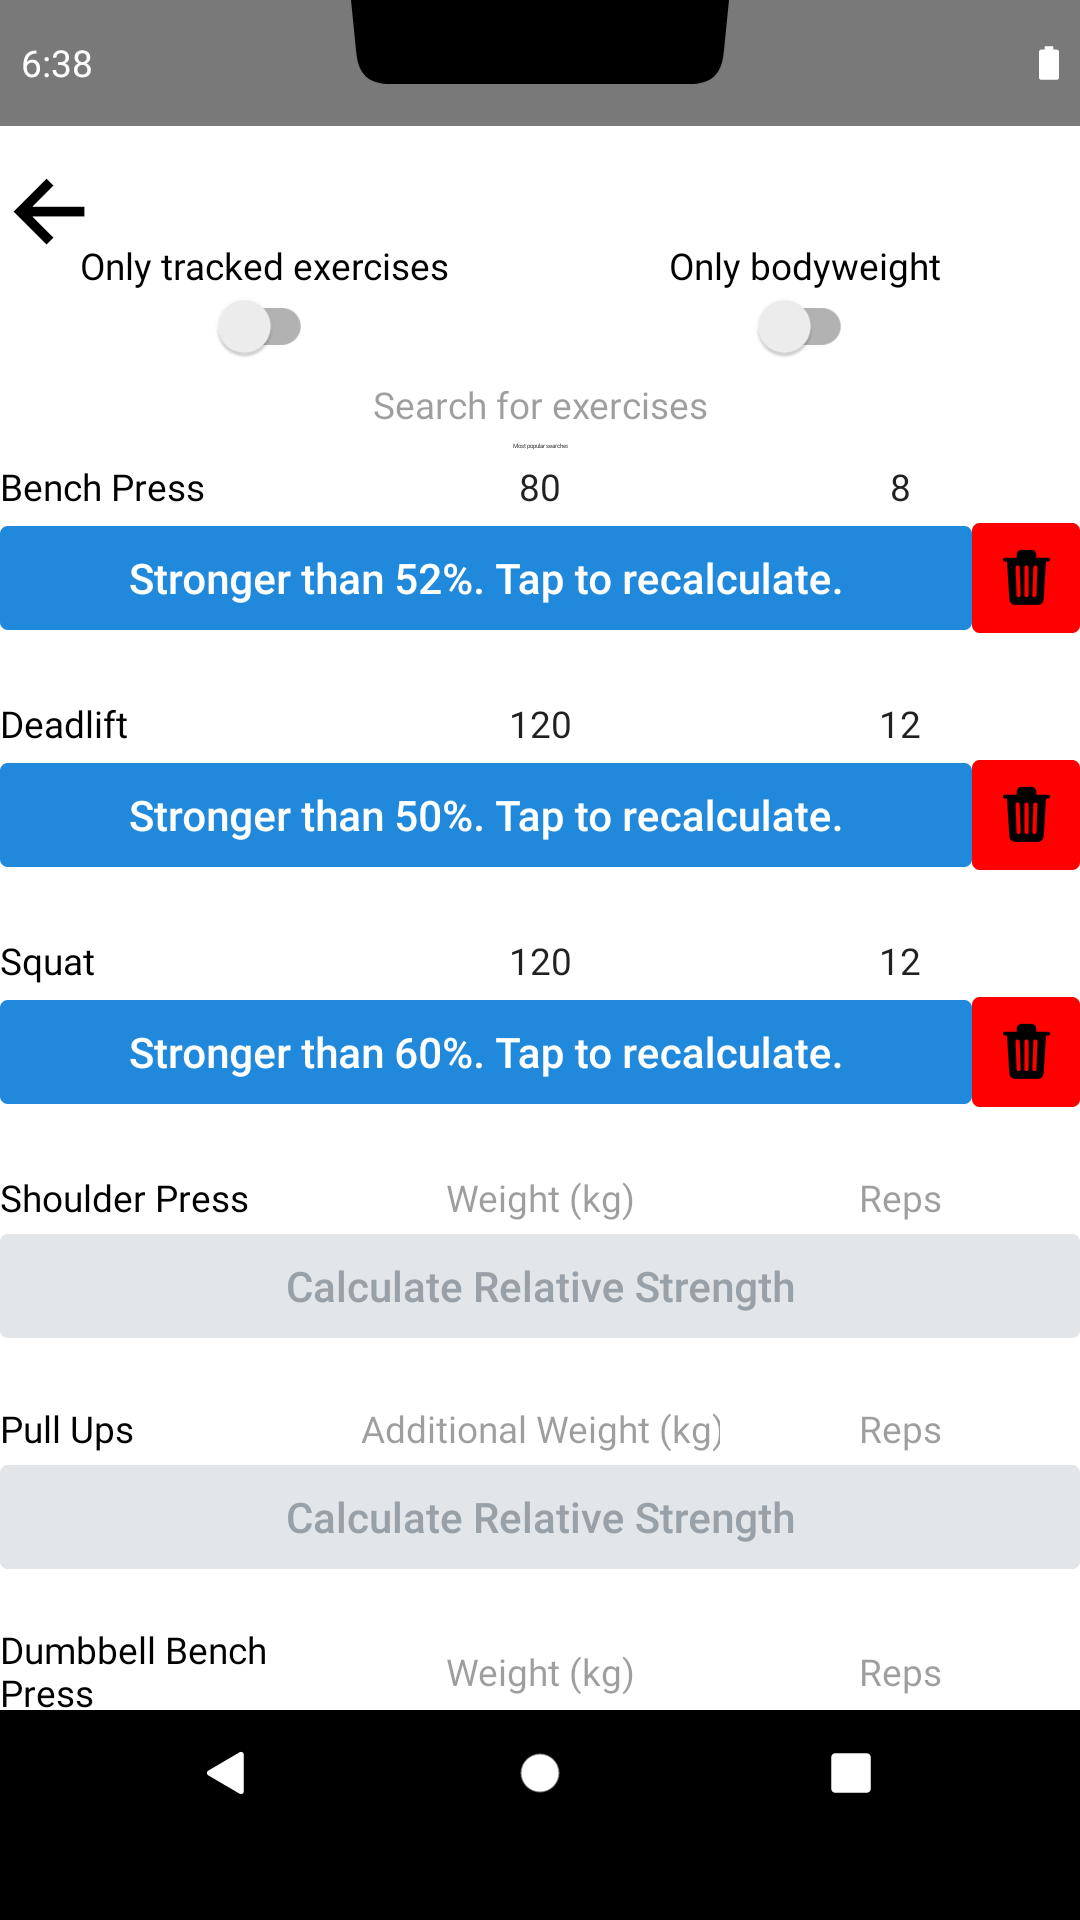
\includegraphics[width=\textwidth]{exercise_modal.png}
        \caption{"Strengthen Character" screen} 
    \end{subfigure}
    \begin{subfigure}{0.45\textwidth}
      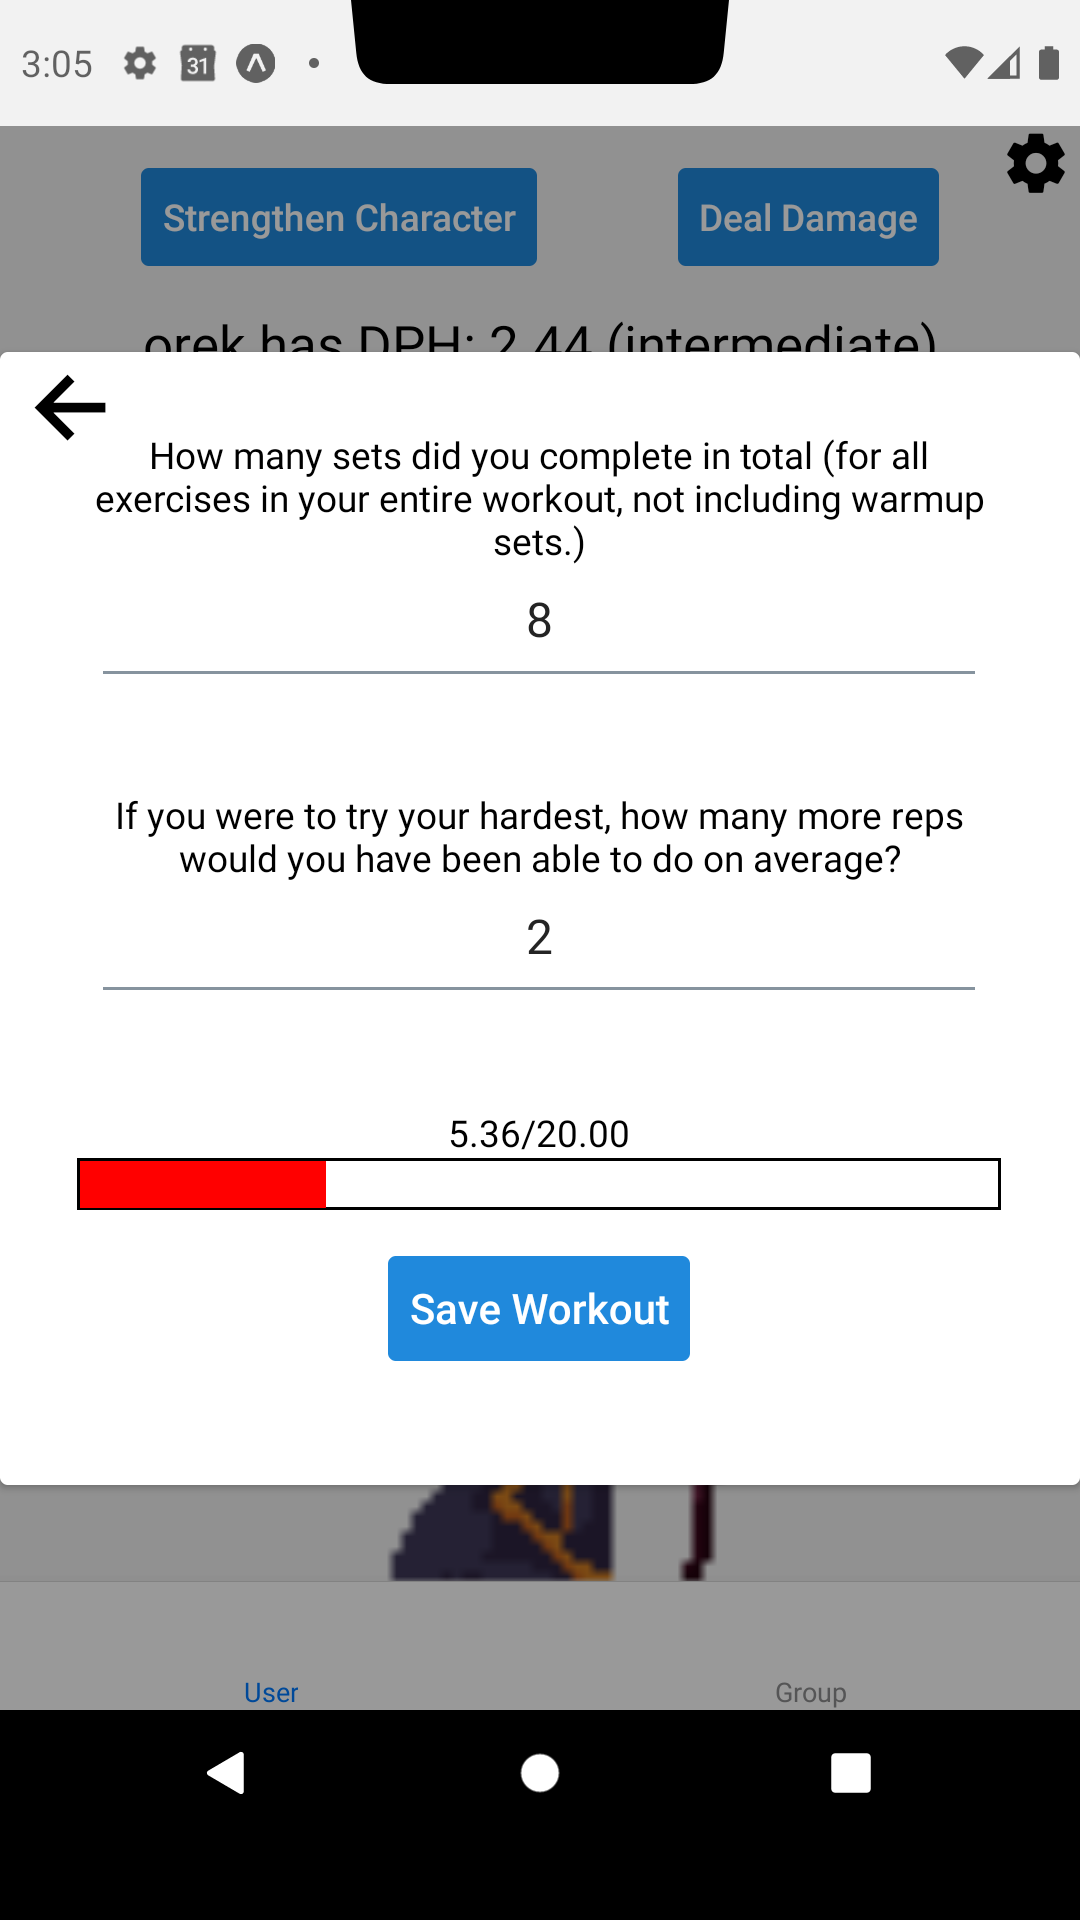
\includegraphics[width=\textwidth]{workout_modal.png}    
      \caption{"Deal Damage" Screen}
    \end{subfigure}
\end{figure}

The right-hand "Deal Damage" screen is far more verbose than the left-hand "Strengthen Character". When I was running my pilot study, I found that participants instantly understood that they were being asked to input how many repetitions of a weight they could do on a given exercise. Users were more confused with the idea of total sets, as they weren't sure what constituted a set. Users also struggled to understand what "reps in reserve" were. I added the explanations above each requested value to help explain these.

I tried to give the user instantenous satisfying and informative feedback. When a user closes the "Strengthen Character" screen after adding exercises, their attack damage changes. Depending on the new attack damage, the character also changes. I wanted everyone to experience this when tracking their first exercise(s). As long as you track a single exercise and make your attack non-zero, you will get a new character. 

\begin{figure}[H]
    \begin{subfigure}{0.45\textwidth}
      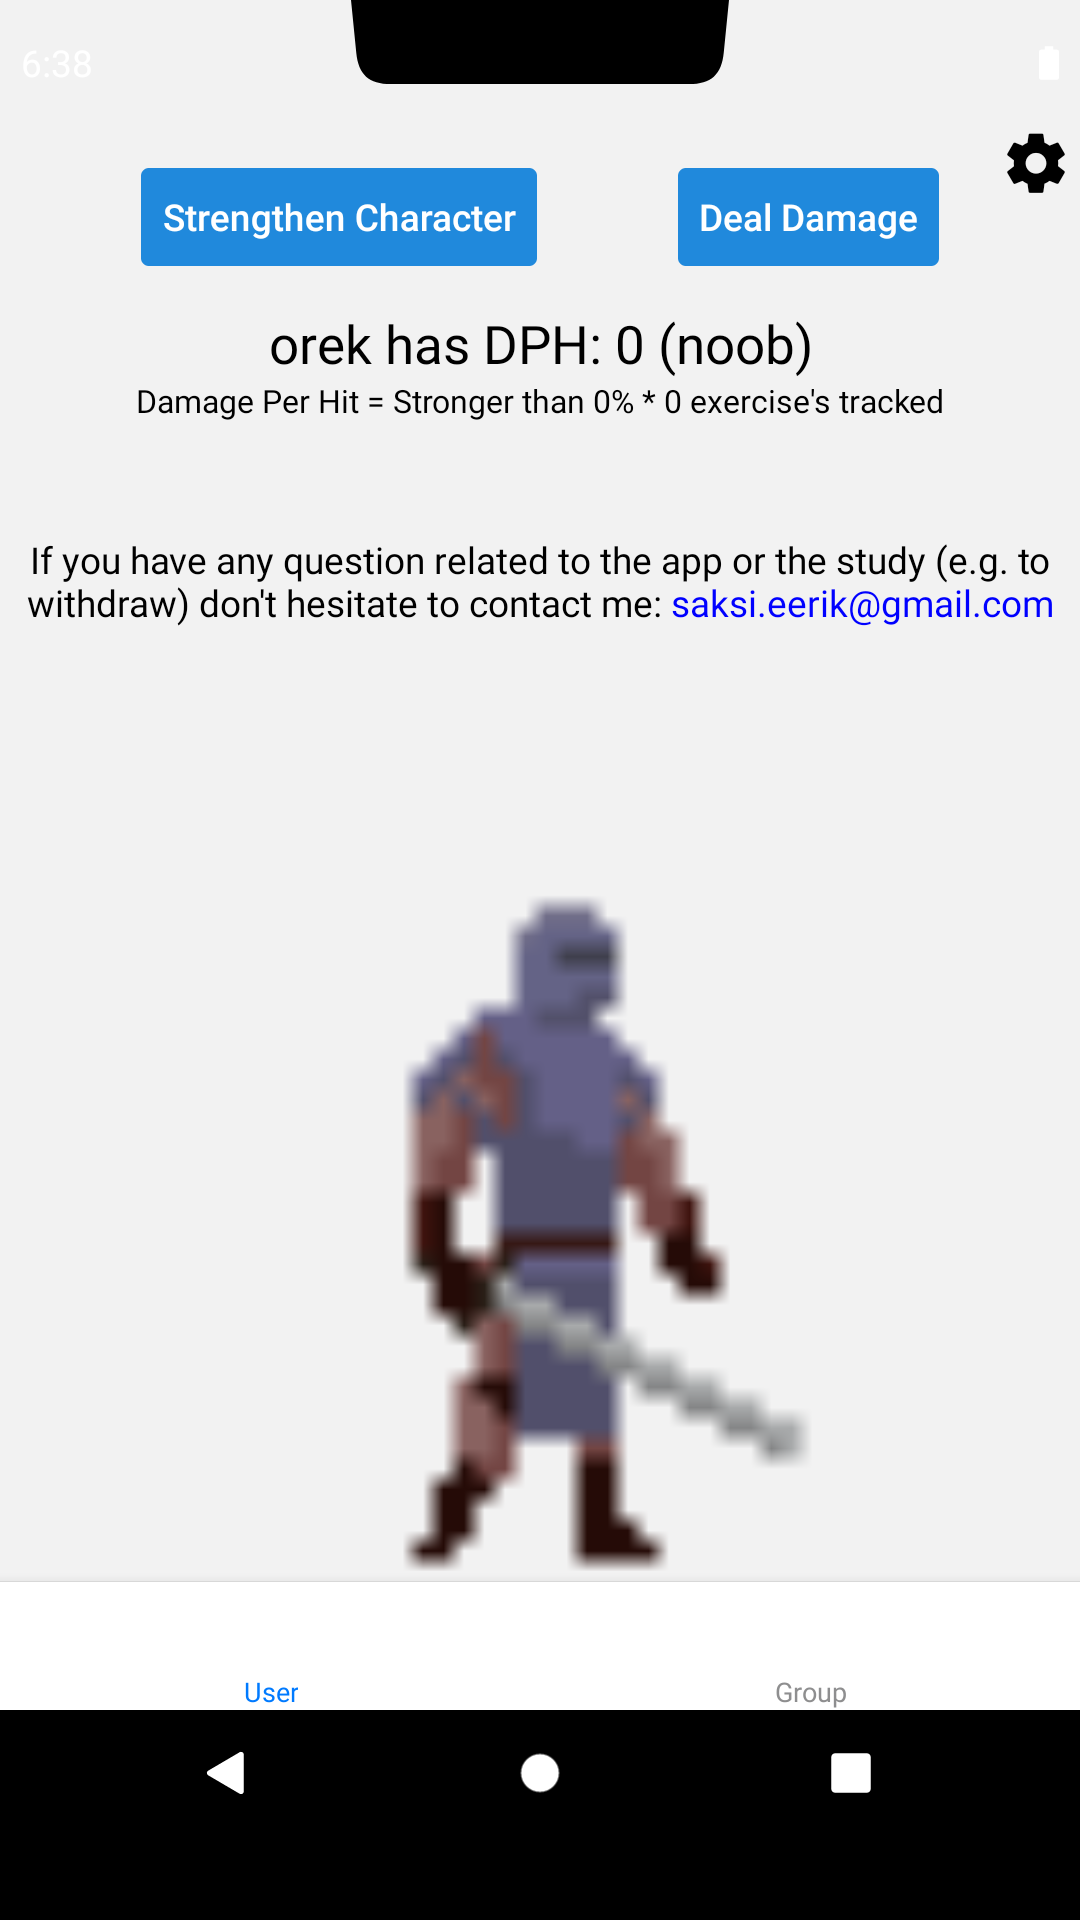
\includegraphics[width=\textwidth]{noob_user_page.png}    
      \caption{What the user sees initially (before tracking any exercises)}
    \end{subfigure}
    \begin{subfigure}{0.45\textwidth}
        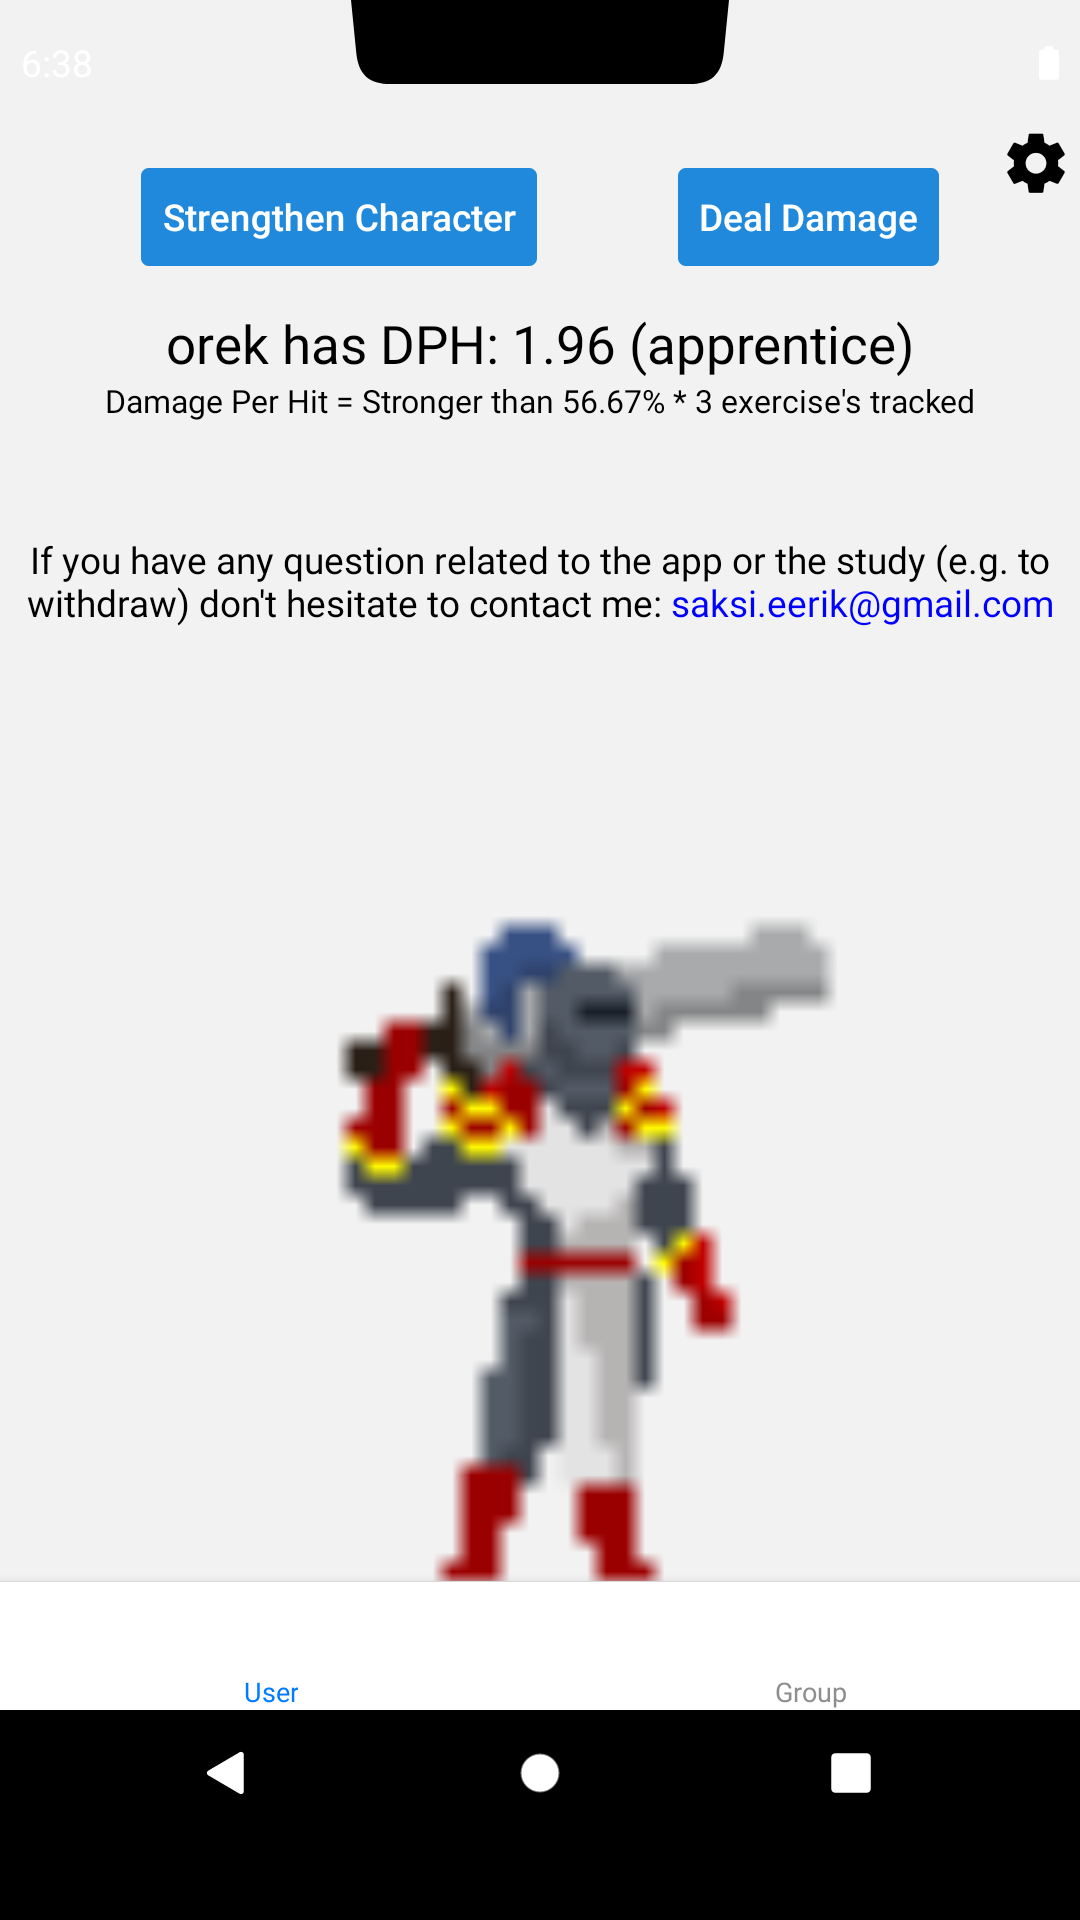
\includegraphics[width=\textwidth]{apprentice.png}
        \caption{What the user sees after tracking 1 or more exercise} 
    \end{subfigure}
\end{figure}

I also tried to make tracking workouts feel satisfying. After saving the workout, you initiate a fight with your team's enemy. You get to see the animations of your character attack, and the enemy take damage, one hit at a time. This is skippable, as it might become boring for long-time users. Killing the enemy will also trigger a dying animation from the enemy.

\begin{figure}[H]
    \centering
    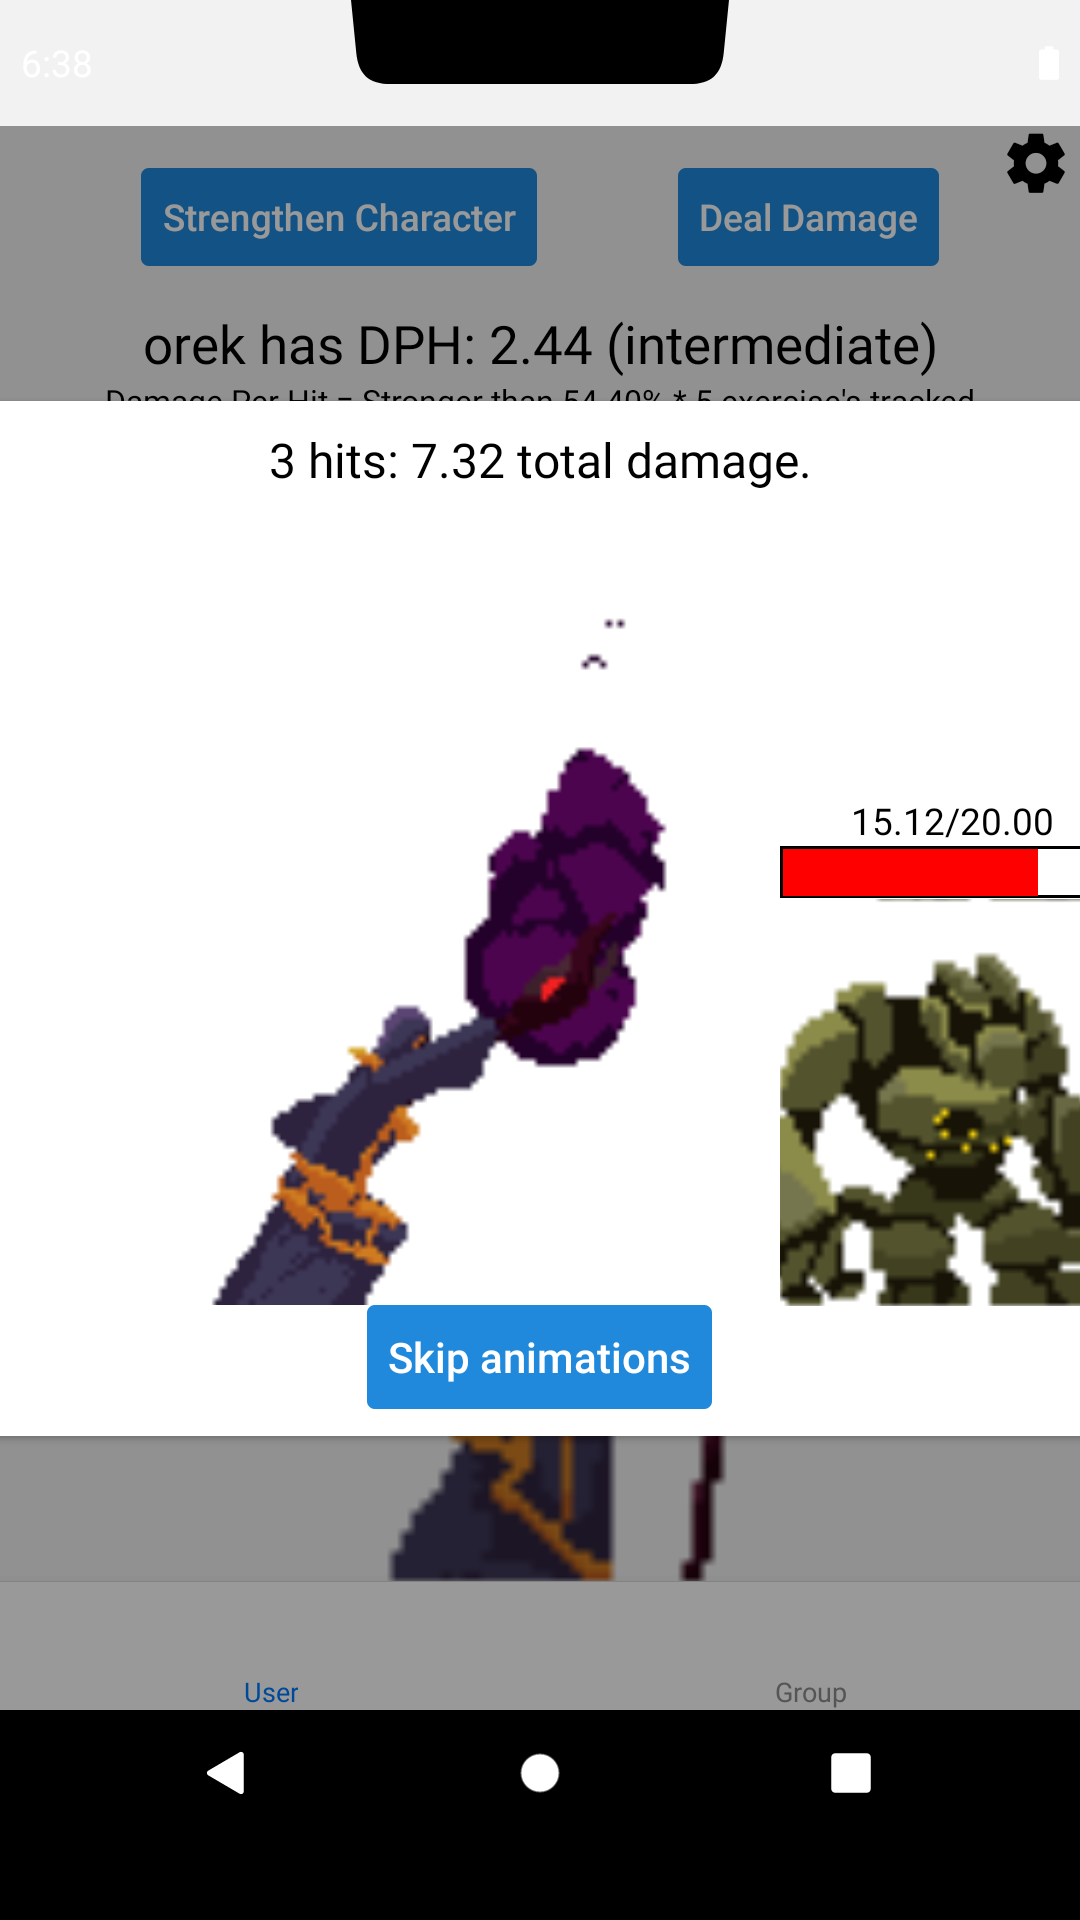
\includegraphics[width=1.0\linewidth]{attack.png}    
    \caption{
      An active battle. There were some visual bugs that I didn't have time to fix.
    }
\end{figure}

I also created a tutorial that explains this idea further. This tutorial is shown when you initially launch the app. In order to demonstrate the connection with real world strength and in-game strength, I simultaneously change real world strength inputs, and the visible in-game characters.

\begin{figure}[H]
    \begin{subfigure}{0.45\textwidth}
      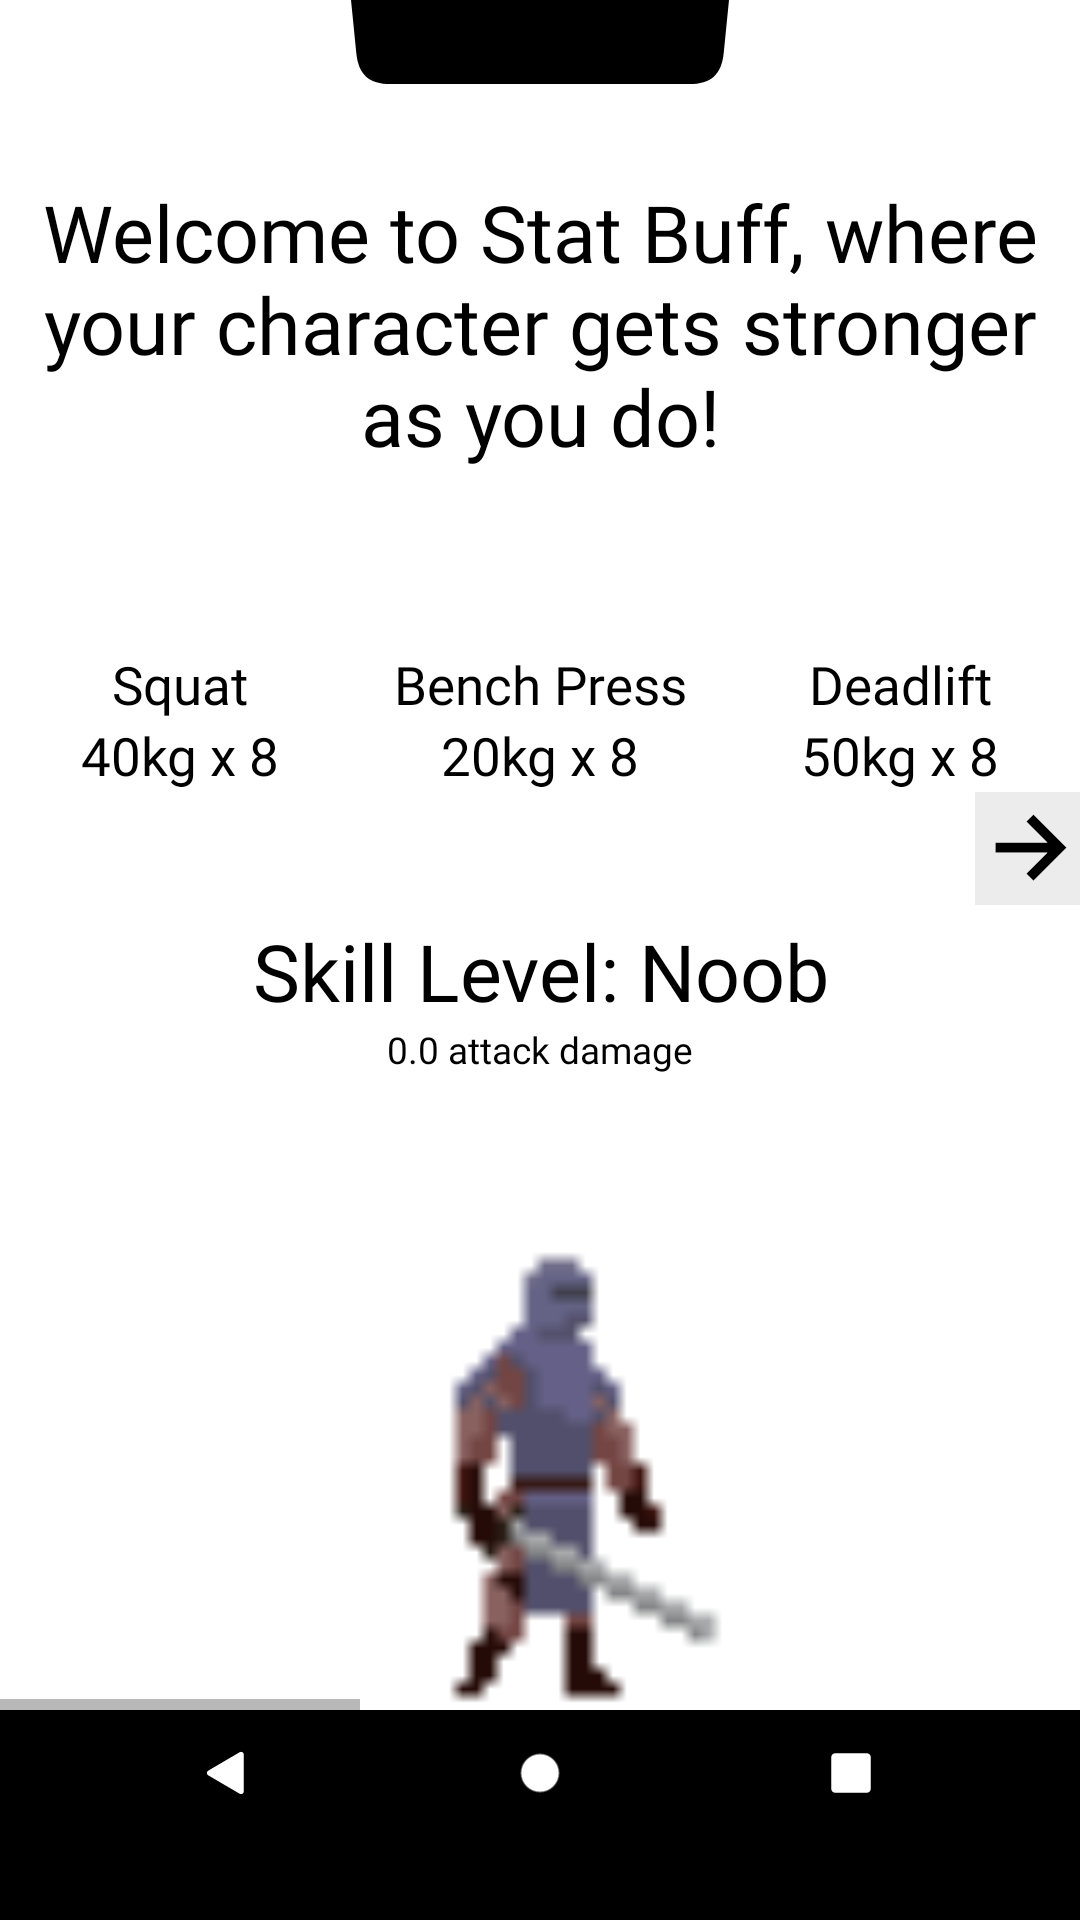
\includegraphics[width=\textwidth]{noob.png}    
      \caption{The first visible character and exercise personal bests}
    \end{subfigure}
    \begin{subfigure}{0.45\textwidth}
        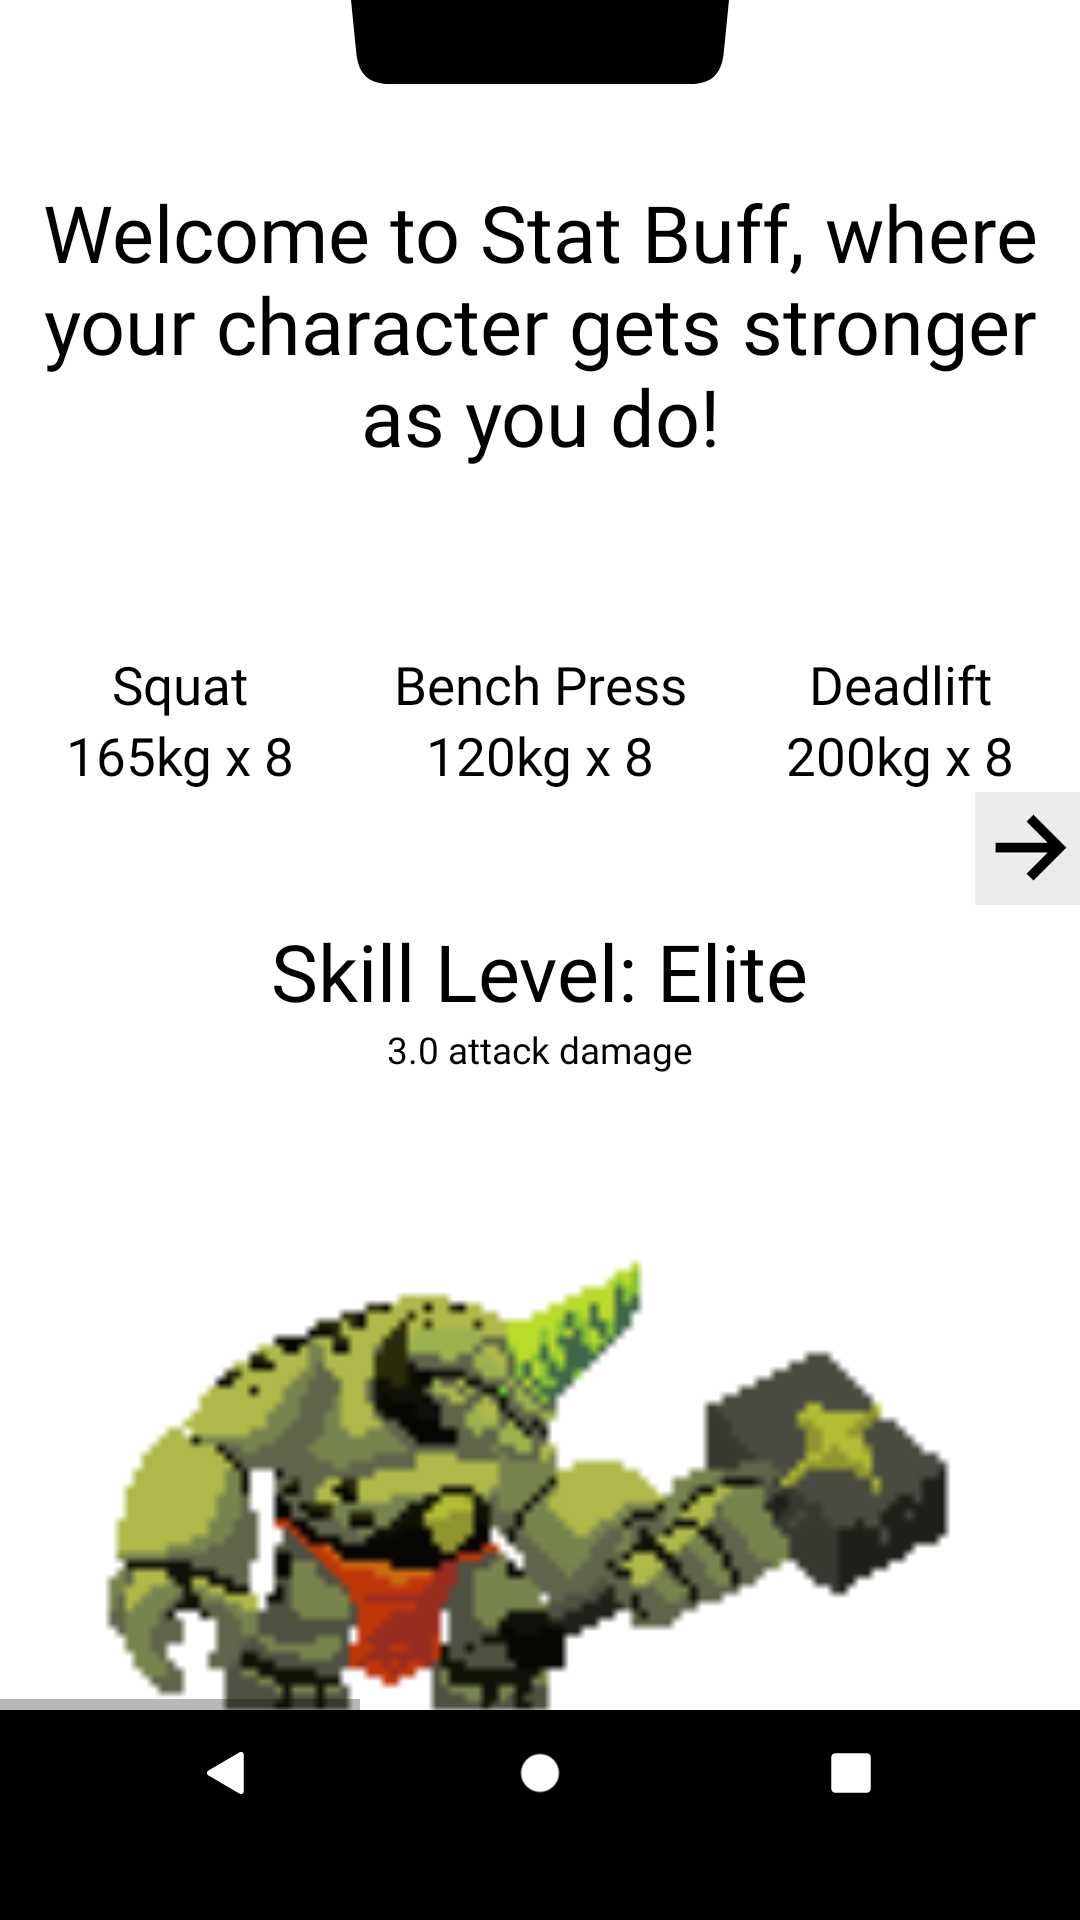
\includegraphics[width=\textwidth]{elite.png}
        \caption{The "elite" character, unlocked through high real world strength} 
    \end{subfigure}
\end{figure}

In order to demonstrate how workouts deal damage towards an enemy that you fight with your friends, I show two different characters take turns fighting a monster, where the second player finishes the monster off.

\begin{figure}[H]
    \begin{subfigure}{0.45\textwidth}
      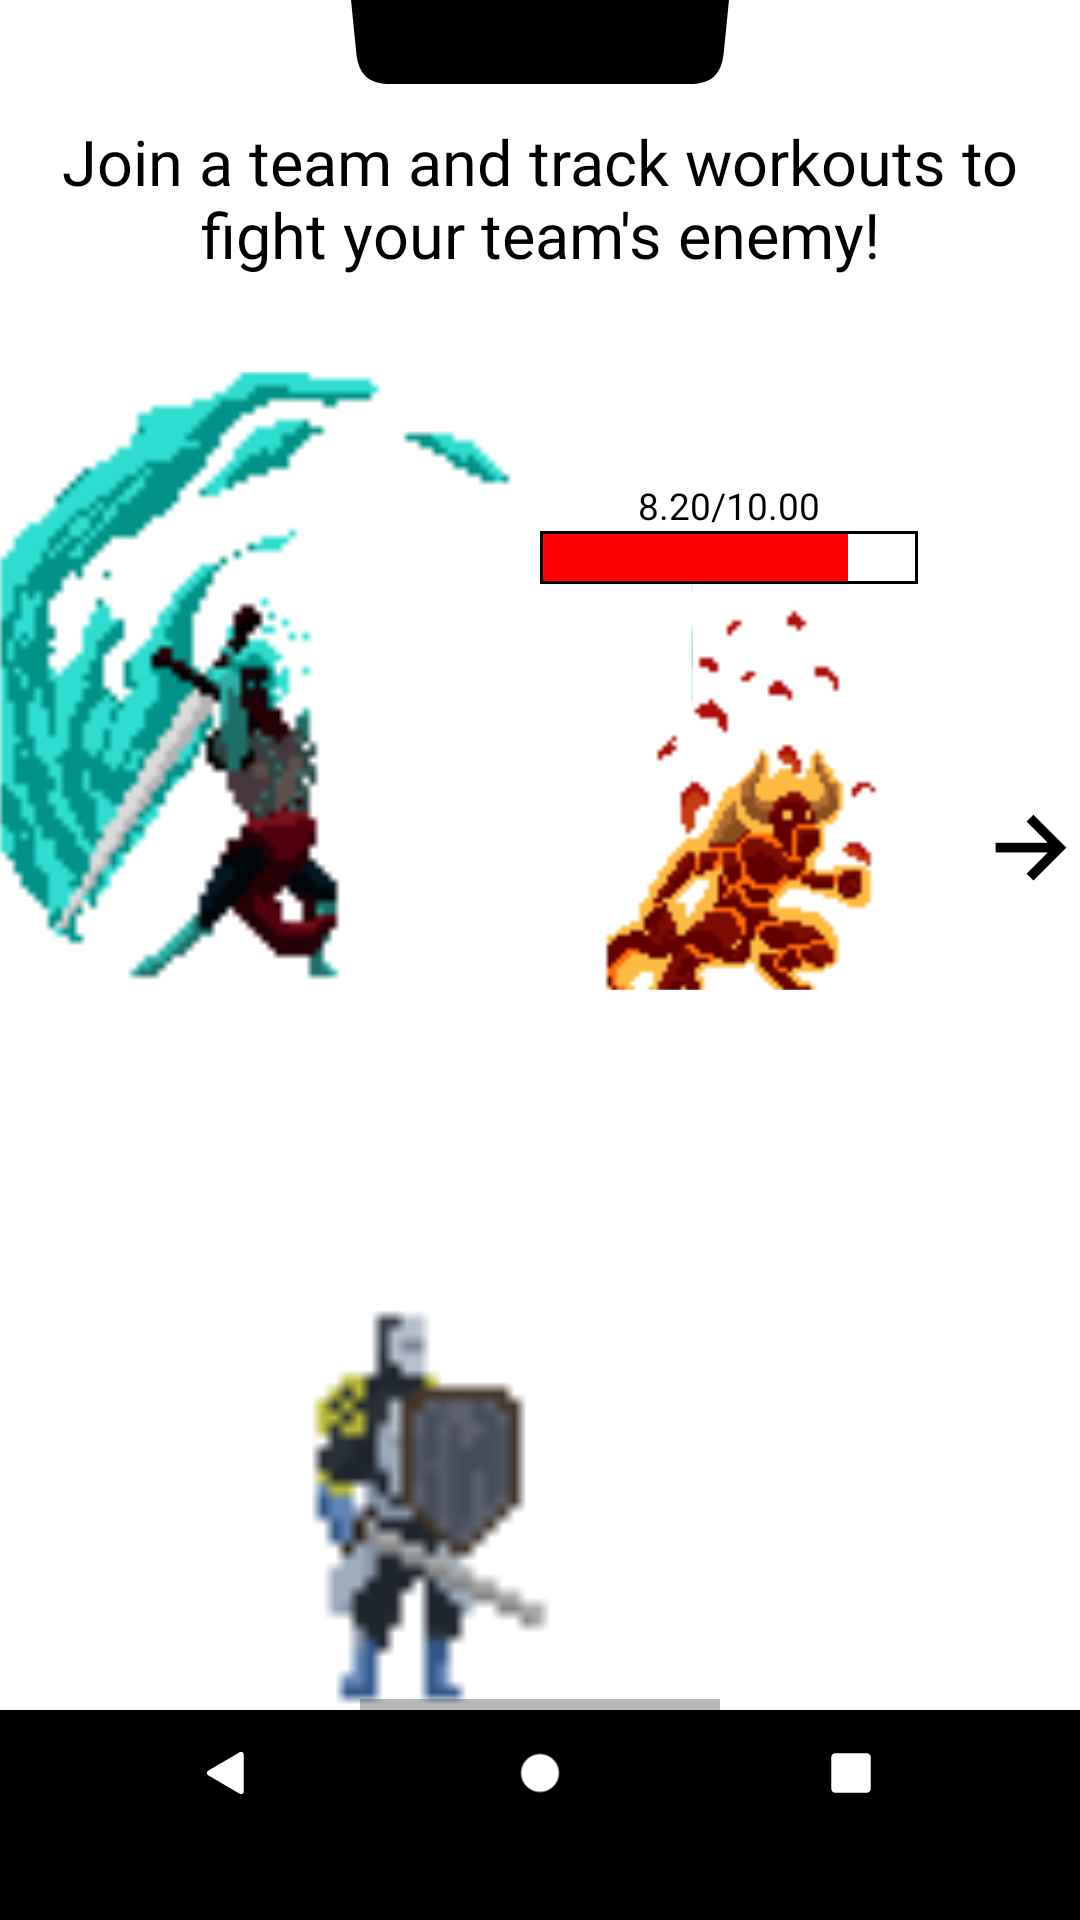
\includegraphics[width=\textwidth]{upper_attack.png}    
      \caption{The first player deals initial damage to the enemy}
    \end{subfigure}
    \begin{subfigure}{0.45\textwidth}
        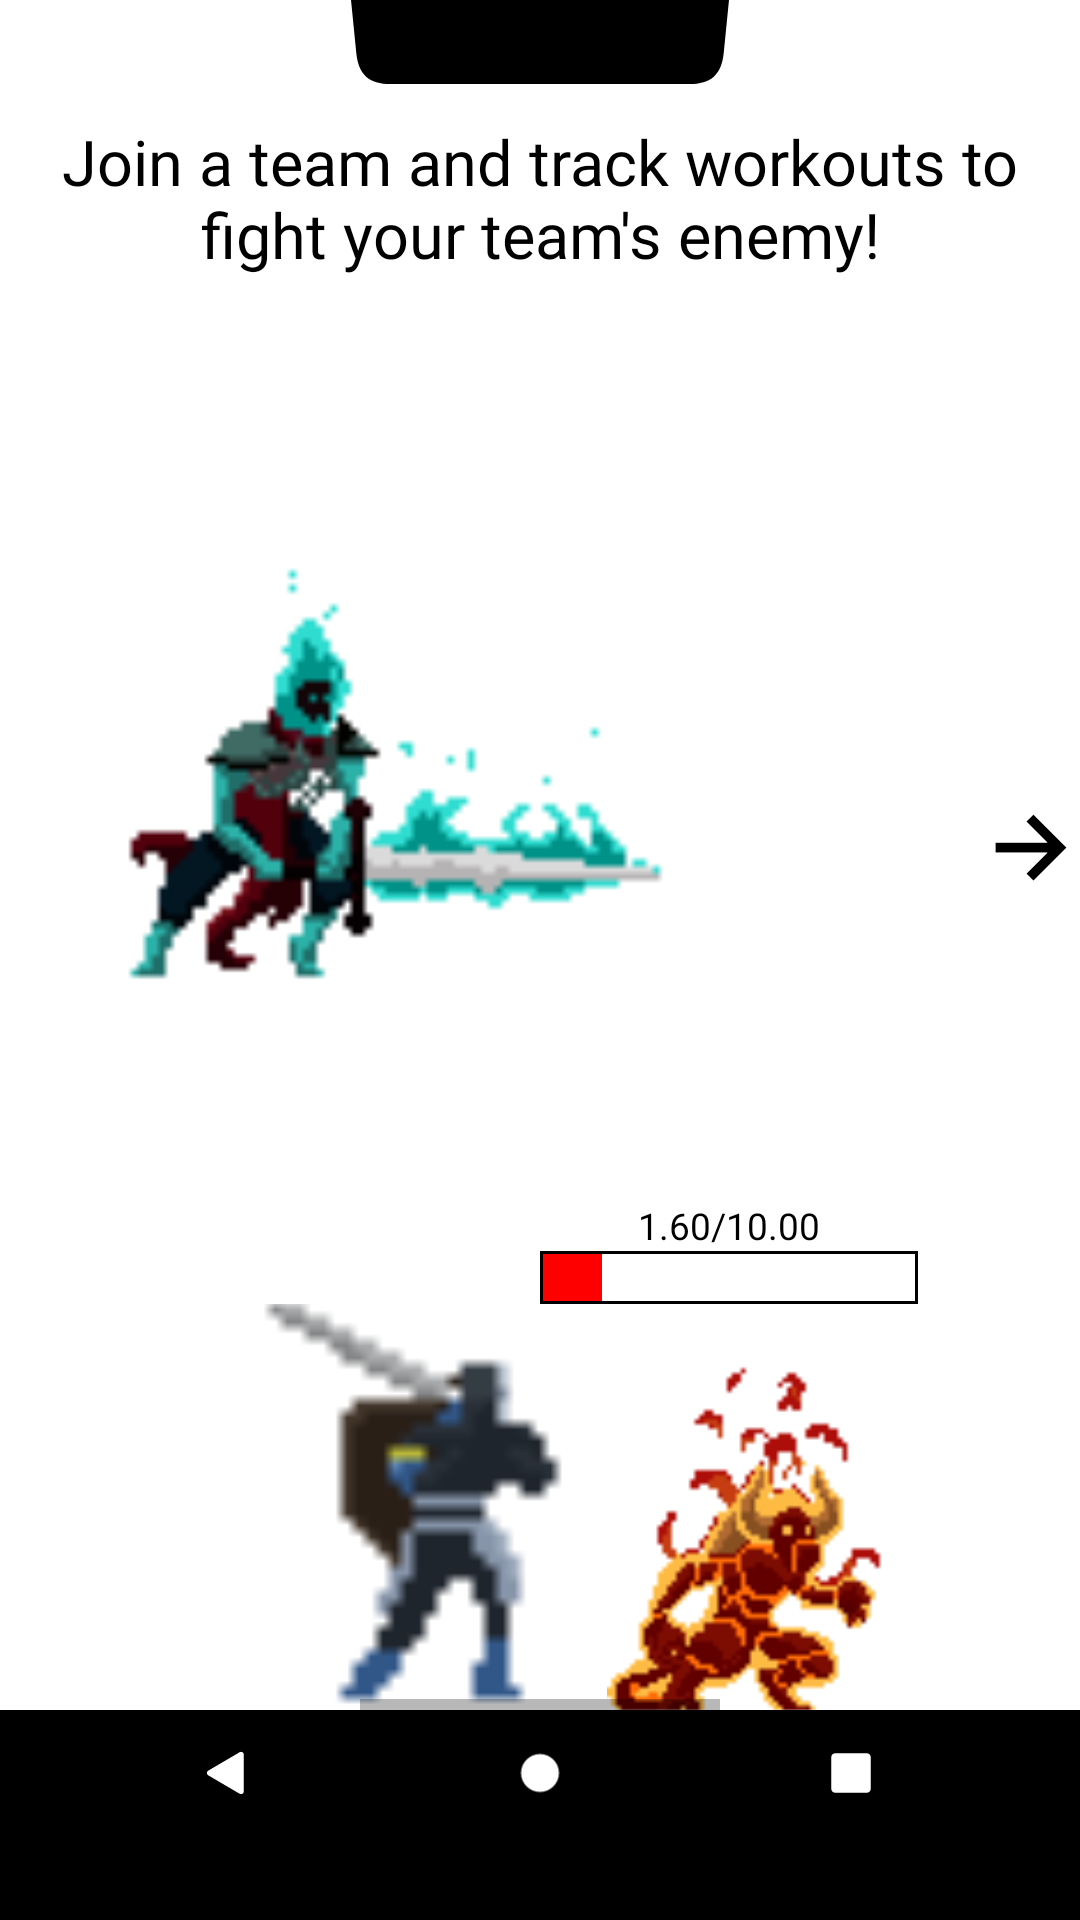
\includegraphics[width=\textwidth]{lower_attack.png}
        \caption{The second player then kills the wounded monster} 
    \end{subfigure}
\end{figure}


\chapter{Implementation}

\section{Technologies that I used}
I first had to choose a technology that I would use to build the client. I decided that an app would be more convenient than a website, as users could enter values during/after exercising. After deciding to make an app, I had to decide which platform's to develop for. Ideally, I would have an app for both platforms, which would allow anyone to participate and to invite any of their friends. I didn't have time to learn how to make an iOS app and an Android app, so I decided to make a single React Native app, which can be compiled into two native apps. I also had some experience, which made learning React Native easy.

As the app was collaborative, I needed to setup a server and a database. I wanted to make this as easy as possible, so I used a technology called Postgraphile, which turns a database into a server API automatically. This technology still required a lot of learning and configuration for the created server to behave as expected.

\section{Server/Database}

The server is built with a technology called GraphQL. GraphQL is a query language similar to REST, except GraphQL requests require you to pass a JSON-like object containing only keys for which you want the values for. This is what a simple GraphQL request might look like: 

\begin{lstlisting}[language=python, caption={An example GraphQL query fetching a user's group}, label=lst:callahan]
  query{
    user(username: "orek"){
      groupname
    }
  }
\end{lstlisting}

\begin{lstlisting}[language=python, caption={Response to above query}]
  {
    "data": {
      "user": {
        "groupname": "Team Public",
      }
    }
  }
\end{lstlisting}
This query format has many benefits: a well configured client would never overfetch or underfetch. In a standard REST setup, the /user endpoint might return user metadata and /messages might return a users messages. This would mean that the client would have to send two requests, which would be slower for both the client and the server. One solution might be setting up a single endpoint, /user\_messages, which returns both user metadata and user messages. This would have the downside of overfetching: whenever we needed just the user metadata, the server would still have to do extra work to fetch messages, leading to a slower query. GraphQL only requires one request to get exactly the data that you need, no more, and no less. The data also comes in the exact shape that you request it in, which makes mapping the data on the client easy. 

This sounds good in practice, but GraphQL can often perform poorly. This was brought to my attention by this video where \citet{Awad} talks about the "N+1" problem. This is characterized by GraphQL resolvers sending needlessly many database queries to fetch data. In order to implement nested resolvers (such as fetching the child books from the parent library) you need to define a function which returns children based on parent values (such as fetching all books whose foreign key matches the parent's ID). In this case, we make one database query to fetch library information, and another one to fetch all books. But what if we fetch all pages of each book? This would lead to potentially thousands of database queries, as each book would call it's child resolver function fetching it's pages. Instead of executing many database requests, this could be executed in a single SQL query by using joins.

Luckily, Postgraphile addresses this. Instead of issuing an SQL query for every single child in the query, Postgraphile acts as a middleware, converting GraphQL requests into a single SQL query. This has huge performance benefits over the afformentioned manual implementation, as only one SQL query is required, and SQL's optimization can be harnessed better (such as through indexes). Another huge benefit of Postgraphile is that it analyzes your databases, and generates your entire query API from attributes and relations in your database. A lot of my time usually goes in to writing, debugging and maintaining basic CRUD server logic. When the database becomes complicated, changing the structure and relationships of your tables requires a lot of work to synchronize on the server. Postgraphile removes all this effort. Postgraphile does require some configuration, as we usually want to grant and limit data access depending on user, and internal logic beyond simply reading and writing data. 


\subsection{Security}
I am used to implementing security logic in the middleware, and not the database, so this was hard for to understand and implement. 

Removing read/write queries from the GraphQL API for specific fields and tables is very simple:

\begin{lstlisting}[language=SQL, caption={This comment tells Postgraphile to omit password fields} ]
comment on column "user".password is E'@omit';
\end{lstlisting}

The difficult part was implementing per user security. When a user signs up, their username is stored along with their salted and hashed password. They receive a JWT token containing their username and a expiry date, which is symmetrically encrypted by a secret key (to guarantee tokens can only be issues by my server). 

%FIX 
\begin{figure}[H]
    \centering
    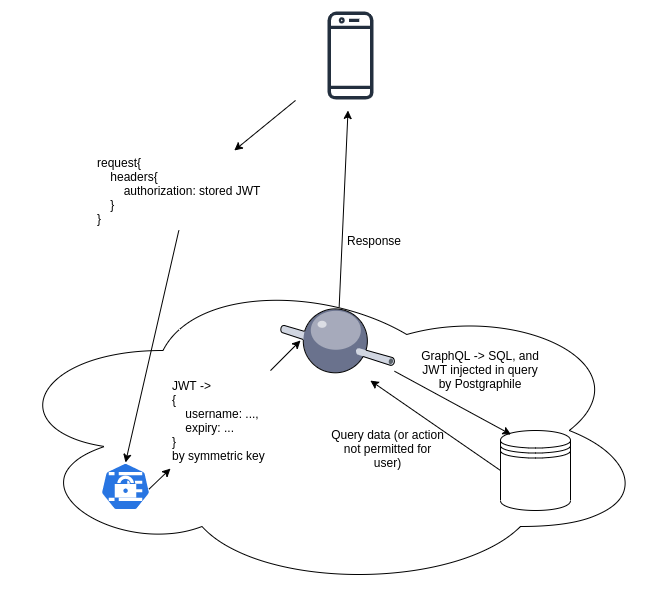
\includegraphics[width=1.0\linewidth]{authentication.png}    
    \caption{
  Once the user has stored the JWT token, this is how authentication works
    }
\end{figure}

Now that the database can authenticate users, it still needs to check whether or not a particular user has rights to perform an operation. This is implemented through row level security policies. Row level security policies only allow operations if the affected row(s) evaluate to true for the supplied boolean expression.

The following code only allows a user to delete or update their own messages. Inserts are only allowed if the user also belongs to the group the message is sent to. Finally, any user in the group is allowed to read their group's messages. This combined with the earlier authentication protects unpermitted data access on the database layer itself. Although verbose, this creates consistent rules that can be written once and enforced everywhere, and prevents bugs that cause data leaks (for instance, you can't accidentally send a group another group's chat messages, as this wouldn't be permitted by the RLS policies).

\begin{lstlisting}[language=SQL, caption={Row level security policy only allowing a user send messages as themselves to their team}, ]
CREATE POLICY chat_message_create ON "chat_message" FOR insert to query_sender with check (username = (select username from active_user()) and groupName = (select groupName from active_user()));
\end{lstlisting}


Finally, I will discuss password management. When a user creates an account by sending an encrypted POST request, I hash and salt the password and store the username in plaintext.

\begin{lstlisting}[language=SQL, caption={Hashing and salting done with pgcrypto}]
insert into "user"(username, password) values (username, crypt(password, gen_salt('bf')));
\end{lstlisting}

Then, when a user requests a JWT token, I simply hash their input password again, and compare it to the stored one:
\begin{lstlisting}[language=SQL, caption={Hashing and salting done with pgcrypto}]
if authenticated_user.password = crypt(input_password, authenticated_user.password) then
  #grant JWT
  #...
\end{lstlisting}

\subsection{Complex database logic}
With the current setup, we can execute simple authenticated rule-based CRUD operations. Usually we want more complex logic. One solution would be to replace the automatically generated queries and mutations with custom written ones that also include side effects. This would go against Postgraphile's philosophy of reducing the amount of source code that needs to be written. I found the best solution to introduce side effects was to use database triggers. Database triggers are functions that execute when specified events occur. Triggers can alter the row that caused the trigger to row, as well as execute SQL that reads/writes from other tables/rows. 


\begin{lstlisting}[language=SQL, caption={Definition of a trigger function which sets the rows' "updated\_at" column to be the current time, and a trigger which calls the function on a user whenever the user is updated.}]
CREATE OR REPLACE FUNCTION trigger_set_timestamp()
RETURNS TRIGGER AS $\dollar$$\dollar$ 
BEGIN
  NEW.updated_at = NOW();
  RETURN NEW;
END;
$\dollar$$\dollar$ LANGUAGE plpgsql;
CREATE TRIGGER set_timestamp
BEFORE UPDATE ON "user"
FOR EACH ROW
EXECUTE PROCEDURE trigger_set_timestamp();
\end{lstlisting}

Triggers reduce the amount of code that needs to be written, as I only need to specify what should be done after a write operation. Traditional side effects also might need to be written more than once: if a user is updated from two different endpoints, both would need to manually update the user's timestamp. Triggers need to be written once, and will always run regardless of what query or SQL statement triggered them.

\subsection{Subscriptions}
In order to implement real time events on the server side, I used Postgraphile's built in websocket subscriptions. Client subscribers listen on a "topic" which is a string representing a real time event source. A topic "blog\_posts" might notify listeners with a link to the new post whenever a new blog was published. In my case, I had topics for every team, which were formatted as "Event\_{Team Name}" (such as "Event\_Dream Team"). The Postgres database alerts Postgraphile when a topic has updated with the pg\_notify() function, along with data about the event itself. Postgraphile then notifies event listeners, along with the information about the event. This event can be a message, a workout, or a new exercise personal record. The client is responsible for presenting the different events. 

\subsection{Other server features}
My server is also responding for sending a participant information/ethics consent sheet. This is a simple React App, containing information about the study and data usage. It requires that the user enters the username which they would like to use and to read and consent to all points. When the form is submitted, the username is saved in ethics consent table in the database. The presence of your username in the ethics consent table is required to proceed with the sign up. This form is opened by the app, which opens the app through once it's submitted through deeplinking. 

\subsection{Deploying}
I originally intended to deploy both my database and server on Heroku, as I was familiar with both. I realized that Heroku's database wouldn't fit my use case: you are not allowed to create roles. My security policy is built on having a super user (which only I have access to) and a restricted database user subject to all security rules. Postgraphile is connected as this restricted user, so any sent GraphQL (and thus SQL) that a user sends is subject to row level security policies. I considered hosting the database and server on AWS, but Postgraphile does not support subscriptions there (due to the serverless infrastructure). I decided to combine the best of both worlds, and used a Heroku server alongside an AWS RDS database (which supports roles, even on the free tier.) It took some work for me to get SSL properly working as I am new to using AWS. Locally, simple CRUD queries only take 10-20ms to handle, and more complex ones such as fetching users by group, and all events by users take 50ms, while on Heroku, this is 60-100ms for simple queries, and 100-200 for more complex ones. I believe that this is partially because of the latency from Heroku to AWS, but I am still happy with the performance, especially for a free server and database.

\subsection{Strength and workout calculations}
A key part of my app is the connection between in game strength and real life strength. Strength is hard to calculate, as it depends on factors such as the exercise, the weight used, number of repetitions, the bodyweight of the user, etc. Although formulas exist for popular exercises (such as squat, bench, and deadlift in powerlifting) I wanted the app to include more exercises, especially bodyweight ones during COVID. I did some research, and couldn't find any API's that handled these calculations, but I did find websites which provided them. I contacted the owners of the sites, and they weren't willing to provide API access. I asked the owner of strengthlevel.com if they would mind me scraping their site, and they didn't. The web client contacts an API to make these requests, and by tracking my network requests when I submitted the form, I could copy and analyze how my request parameters were sent. I then made the exercise request generalizable (for instance, by changing the exercise which I submitted, "barbell-squat") to the variable exerciseName. The node.js server didn't allow for the Strength Level request to be made, as it wasn't encrypted. After doing some research, I found two solutions: one would be to disable this restriction and to send the request without any encryption. This is a bad idea, as the request contains some sensitive information (exercise performance, identified gender, weight). This would also remove warnings when sending unencrypted requests to other hosts. The latter solution involved getting the public key (.pem file) of Strength Level, and encrypting the request with it. This was harder, as I didn't have experience with this, but I'm glad I learned to do it properly (as I also needed to configure Amazon's public key for database requests).

Most of the request parameters were self explanatory (exercise weight, bodyweight, repetitions, etc.) as it was obvious that they were just numbers. The exercise name parameter required more work to generalize, as this was a string which had to be in the small subset of supported exercises. I scraped the names of this by copying the HTML of the exercise browser, and by stripping everything but the names. This was initially enough information to set up relative strength calculations. Months later as I tracked a bodyweight exercise, I found that the request didn't work. This is because bodyweight exercise have a different query format. Instead of requiring lifted weight as a parameter, they require "additional\_weight" and "is\_bodyweight". To accomodate for this, I added an extra field to all exercises (is\_bodyweight), scraped all exercises tagged as such, and set is\_bodyweight to true for all those exercises. I also had to refactor the request sent to Strength Level depending on if the exercise was a bodyweight one or not. After fixing this bug, it was very easy to add a "bodyweight only" filter to the exercise search in my app, which hopefully made my exercise. 

I accidentally mislabeled two exercises as bodyweight, which lead to one user's client repeatedly crashing. My server threw an error, as Strength Level didn't give a valid response from the malformed request, which lead the user to receive an error aswell. The client would try to resend it whenever they relaunced the app, which lead to more crashes. I fixed these exercises in the database, and told the user to remove their cache (which stopped the user from trying to send a malformed request).

I wanted groups to be able to search exercise updates by user for particular battles against monsters, or all battles. One simple solution would be to select based on timestamp (if a battle against a monster started 2 days ago, select all exercise updates where the "created\_at" attribute is less than 2 days from now). I decided not to do this, as this would be very slow since the timestamp is not an ordering attribute. Selecting all matching exercise updates would require searching all of the user's updates. Instead, I decided to add nullable foreign key attributes, battle\_number and group\_name which denote the battle in which this exercise was tracked, and the group in which the user belonged to at the time. This metadata is not sent by the client, but read and written by a database trigger after the user inserts an exercise personal best. This trigger might not do anything, as the battle\_number and group\_name returned from the query might be null.

\begin{lstlisting}[language=SQL, caption={This selects the group and battle of the user that created this exercise update}, label=lst:trigger_set_metadata]
select group_name into NEW.group_name from "user" where username = NEW.username;
select battle_number into NEW.battle_number from "group" where name = NEW.group_name;
before insert on "user_exercise"
\end{lstlisting}


Using foreign keys allows us to construct queries GraphQL which fetch exercise updates based on group or specific battle, as Postgraphile recognizes relations. Loading the group's name into the exercise update also makes it easy to set up subscription updates. I use the group's name field to alert the corresponding group of this event.

I also load the battle and group foreign keys into workouts, but these fields are mandatory. Tracking workouts makes you deal damage towards your enemy, which doesn't make sense if you don't have an enemy. On the other hand, you can strengthen your character without needing an active enemy. I calculate the number of granted hits using a simple generated column:

%\begin{lstlisting}[language=SQL, caption={Calculate hits based on user supplied average_rir and sets}]
%hits integer GENERATED ALWAYS as ((10 - average_rir) / 10.0 * sets) stored
%\end{lstlisting}


I also needed to calculate the damage that this workout dealt, and to subtract the dealt damage from the current enemy. To do this I needed to implement a trigger that activates whenever a workout is created. This trigger first calculates the total damage that this workout dealt by multiplying the number of hits with the attack damage of this user. I then subtract the current health from the group's enemy. Finally, I check if the health of the enemy is 0 or less, in which case I progress the group forward by one level, giving them a new stronger enemy at full health. A team might not always succeed in killing the enemy within the allocated week. Whenever a user fetches data about their team's enemy, I check whether or not this current battle was created over a week ago. If so, I create a new battle with the same enemy, but everything reset (1 week to kill and full health). I also send the team a message to their group chat notifying them that they failed to defeat the enemy, and that it has been reset.


\section{Client}
\subsection{Framework}
Since the app was collaborative, I wanted users to be able to invite any of their friends to participate. I didn't want there to be any technological barriers to entry. As most people in developed countries have an Android or iOS phone, I decided that a cross platform app would be best suited for this, and would allow users to use the software as they trained, as opposed to a desktop app. 

As I already had some experience with React, I decided to use React Native. There are some differences, mainly that the DOM that components use different tags (a basic container is called a View as opposed to a div). I quickly realized that React Native isn't simply about developing one code base. When installing some libraries, you would need to configure the Android Kotlin code, or the Swift code of the iOS app. I was intimitated by this, as I had experience with neither language or build system. Another issue is that I was developing on Linux: testing and building the iOS app was difficult, so I wanted the iOS app to stray from the Android version as little as possible.

I decided to use Expo, which is a superset of React Native. You can create a React Native app through Expo without touching a line of platform specific code. Expo also handles certificates and keys for you, which was enticing, as I didn't even know what they were. It is also easy to convert back to React Native if I wanted to. Expo has some issues, but so does React Native. 


\subsection{Performance considerations}
React Native apps compile into platform specific classes and components, eg. a React Native <View/> component becomes a Swift UIView on iOS, and a Java/Kotlin View on Android. Any Javascript that you write, or Javascript libraries that you use will stay as Javascript. React Native allows you to compile custom binaries which written in languages such as C, but Expo does not. Javascript is a slow language. It is not compiled like native app languages, and instead interpreted. This could prevent some older devices that already have performance issues from my app. In my case, the app was reasonably simple, and much of the data processing was handled server side, so this was not much of an issue. 

\citet{app_size} compared the sizes of different APKs generated by Java and React Native. A simple app that showed "Hello world" to the user 539 KB, while the React Native app 7 MB. This is primarily caused by the bundled Javascript interpreter which the React Native app bundles along with the App. This is not a requirement for Java apps, as Android devices come bundled with Java Runtime Environment. App size only gets worse with Expo: "An application with Hello World weighs 25 MB" \citep{expo}. App install size is very important: "For every 6 MB increase to an APK’s size, we see a decrease in the install conversion rate of 1\%" \citep{app_conversions}. This article primarily stresses the importance of app size when developing apps for countries with poor network connectivity and cheaper devices. My participants primarily resided in Finland and United Kingdom, where storage and network connectivity isn't as much of an issue. None of my participants reported that they couldn't install the app. There is also a difference with download and install size: The Android App Bundle (aab) is about half the size of an APK to download, and this bundle is also compressed. My app download size was about a fourth of the install size.

One of my primary concerns was the startup time of my app. A device must first load the "Javascript Bundle" which is a file containing all of the Javascript of the app. This is usually unnecessary, as an app has multiple screens and sections which are only required when these screens aer opened. With this default behaviour, my app took 5 seconds to open. This gives bad first impressions, and might make some users think that hte app has crashed. Slower startup times would also increase the barrier of entry for tracking workouts and engaging with your team, which would reduce app use significantly.

In order to alleviate this, React Native allows you to load the bundle component by component as they are rendered. A custom placeholder can be rendered as the component loads. This also reduces the load on the server: components which send requests only do so when this data is needed. Every modal and overlay is only loaded into memory when it is opened and the group tab is only loaded once the user has navigated to that tab. One of the most important lazy imports that I implemented was for the app and the app demo. The app demo is only needed if the user hasn't signed in. Conversly, the app is only needed after the user has gone past the app demo and signed up. One issue with this implementation is that we need to receive a server response validating that we are signed in and that our JWT token hasn't expired before we can decide which component to load. 

Luckily my query client, Apollo, has a solution for this. You can configure Apollo to cache queries in the devices' local storage. When executing a query, Apollo initially returns the data that the server responded with last time. Once the server sends the response, Apollo mutates it's returned data. When the local storage of the device matches the server, the query is unnoticeable, as Apollo does not update the rendered local data. When the data is out of sync, you briefly see outdated data before seeing new, refreshed data. It is relatively rare that the login status is out of sync with the server, as my JWT's expire every two weeks. In this case, the device loads the main app into memory, after which the user is taken back to the login screen. I use caching for most of my other queries as it doesn't require me to compromise between staying synced with the server and making the user wait. There were some cases where this caching policy lead to accidental features. When you open your team tab to view the state of your monster, you initially see the monster sprite and the health when you last viewed it, before the health/monster updates (if other users worked out while you were gone). This shows the user of the progress that was made while they were gone.

Apollo's cache also leverages Postgraphile's "globally unique identifier" implementation. This concept was introduced by another query client, Relay. A globally unique identifier is an identifier which is not only unique for a particular type, but for all types. For instance, a user and a group cannot have the same globally unique identifier, even if some have the same primary keys. Postgraphile implements this by sending a base64 encoded string containing the name of the type, along with the primary key of the type, which is unique for all rows for all tables. This allows Apollo to merge data more efficiently, and to refetch data more sparingly.


\subsection{Development techologies}
I used Typescript during my development of the app, which is a superset of Javascript containing type checking. Typescript is not shipped with the app: it is compiled into Javascript. Javascript was designed to absorb errors in production, which is good, as a slightly malfunctioning app is usually better than a crashed one. Typescript enforces what Javascript does not enforce in development, such as null checks, supplying required parameters, and more. All parameters supplied to React components are optional in Javascript, which can lead to errors being thrown by the child component and not the parent which neglected to supply a required parameter. Typescript also enforces the types of the parameters, which prevents weird type issues which Javascript is often known for.

\subsection{Analytics}
In order to better understand how the client was being used, I setup simple analytics tracking. Whenever a user opens an overlay or navigates to a screen, it sets a global visibleSection variable to it's own name. I set up a listener for this global variable, which pushes the new section to the end of a list whenever the visible section changes. I also append the total time spent on the last section. I set up another listener, which sends the path that the user took around the app when they close the app. When the analytics are sent, the path is set back to an empty list to avoid sending the same path twice.

\subsection{Sprites}
In order to make the app more lively, I bought a sprite pack from an artist. I ended up using 6 different characters, and 8 different enemies. The sprites had varying amounts of whitespace around each frame. This made it difficult to center elements consistently. Fights would look weird with the enemy, as they wouldn't be centered vertically. I tried to solve this by applying absolute positioning to the characters, but this would break depending on the device. Eventually, I removed the whitespace from the sprites manually. I made a bash script with ImageMagick, a command line image editing tool. Each frame of the sprite sheet needed to stay the same size. My script required the number of rows and columns in the sprite sheet in order to calculate the size of each frame, as well as the percentage that should be clipped from the top, left, right, and bottom of each frame. This was a bit tedious but it worked.

In order to make the characters idle, I simply had to loop the idle sprites. In order to make the character battle with an enemy, I triggered the player animation, which had an onFinish() function hook. The player's onFinish() call triggers the enemy to trigger it's "on hit" animation. The onFinish() call of the player triggers the enemy to attack again. This repeats until the enemy is dead, the player has no more attacks, or the player skips the animations.

The server sends the name of the sprite that should be rendered, but the sprite is stored on the client's device. The server classifies the user's strength, which tells the client which sprite to render. The server also tells the client which enemy it should render in the team view.


\subsection{Deploying}
Deploying the app to Google Play was very easy. I had done all of my development with an Android device, so I didn't need to do extra testing. My first production build was accepted. It took a few days to make sure that everything was working as expected on iOS. I primarily had to make sure that text sizes and buttons were well sized for Apples flagship phones, and that safe area views were working properly. I also had to take screenshots with multiple devices, create a privacy policy, and do just about everything I did for Google Play again. 































\section{Guidance}
You can't talk about everything. Cover the high level first, then cover important, relevant or impressive details.


\section{General points}
These points apply to the whole dissertation, not just this chapter.


\subsection{Figures}
\emph{Always} refer to figures included, like Figure \ref{fig:relu}, in the body of the text. Include full, explanatory captions and make sure the figures look good on the page.
You may include multiple figures in one float, as in Figure \ref{fig:synthetic}, using \texttt{subcaption}, which is enabled in the template.


\subsection{Equations}

Equations should be typeset correctly and precisely. Make sure you get parenthesis sizing correct, and punctuate equations correctly 
(the comma is important and goes \textit{inside} the equation block). Explain any symbols used clearly if not defined earlier. 

For example, we might define:
\begin{equation}
    \hat{f}(\xi) = \frac{1}{2}\left[ \int_{-\infty}^{\infty} f(x) e^{2\pi i x \xi} \right],
\end{equation}    
where $\hat{f}(\xi)$ is the Fourier transform of the time domain signal $f(x)$.

\subsection{Algorithms}
Algorithms can be set using \texttt{algorithm2e}, as in Algorithm \ref{alg:metropolis}.

\chapter{Evaluation} 


I had a total of 24 participants. Participants were recruited through messaging apps. I usually only mentioned that I was conducting research on an exercise app, and nothing more. My app had built in tutorials, and required that users signed a participant information/ethics consent sheet, so I didn't need to give much information about the app. After three weeks, users were asked to participate in a survey.


Interviews take much longer than surveys, as you have to schedule conduct, transcribe, and analyze them. I only interviewed 10 people. In order to maximize the value of each interview, I classified users in to different categories, and sampled from each group. Some users belonged to more than one category. 

Some users had some issues with exercise inputs being removed. This bug was hard to reproduce, and probably had to do something with parent component refreshing. 

\subsection{Strongest members of teams}
Two users that interested me (User 1 and User 3) were the users that contributed a substantial amount of the damage to the team (80\%+). Both the users had a lot of training experience. User 3 was the strongest out of all users, and User 1 was above average in strength, and had used an activity tracker named "FitNotes" before. I was interested in what drove them to contribute such a large amount, and how they felt about doing so. 

\subsubsection{Motivation}
Both of these users mentioned competitiveness, but hardly anything about collaboration. It is hard to say whether or not competitiveness drove these users to perform better, or they became competitive once they realized that they were well. For instance, User 1 suggested a feature: "you could click it and see all the movements that they did in the gym, and the weights and the like the reps. I think it would be a bit more interesting. And for people who like competition it would be fun.". User 1 wanted more transparency towards other members' actions, so that he could compete better. User 3 thought that being able to see the damage and actions of other users leads to competitiveness and more actions "Oh, ****, User 3 is out there, I've got to do the same". 

\subsubsection{Reaction towards being the strongest}

User 1 and User 3 had very opposite reactions towards being the best. User 1 commented: "If everyone would have been contributing equally, I think I would've put much more effort into it." At one point, User 1 had sent a chat message asking if the other member's had gym access. He later explained that this was a passive agressive way of asking why the other users weren't contributing enough. 

User 3 reflected on his gameplay with "Plus, I was carrying those noobs." in a satisfied tone ("Carrying" in games refers to single-handedly winning games for your team, and "noobs" are beginners). Although he clearly enjoyed being the best in his team, he didn't think it would be fun if it someone else was outdoing him by a large margin: "And then we had one guy who was working out seven out of seven times a week for three to four hours a day. And so imagine that we had that guy in our team: he would be doing like 90\% out of a team of 10 people." 

Both users suggested fixes to balance the user contributions. User 1 suggested that the game should rely on each team member more, by dividing users into different classes with different responsibilities. "You will even have a kind of social pressure to do a workout. If your team's success is based on your stamina stat or something like that." I had considered increasing per-user responsibility more. I decided not to do this, as I didn't want to unactive users to prevent progress, but only to slow it down. I asked this user how they would feel if they had to rely on someone who was not active. User 1 responded: "If my progress in the game would be relying on someone who doesn't do anything. I think it would be a bit unmotivating for me." 

User 3 had a suggestion that involved changing how the game behaved, rather than how user actions should be influenced. He suggested: "Bonus damage, which might be the adjusted percentage of the monsters health. So it doesn't matter how weak you are, you could still offer the team that percentage damage". This would mean that everyone's effort would be equally valuable. Users would still contribute more to their team through being stronger, but this would allow weak users to contribute equal amounts in at least one dimension. 


\subsection{Team's composed of strangers}
By default, my app allowed the creation of one person teams. I decided to prevent this feature, as I didn't want many single-member teams to form, as these users wouldn't be collaborating with anyone. I didn't want users to drop out if they didn't want to invite friends, so I added a "Join Random Team" button, which would place you in the smallest and oldest public team. This lead to teams with 2-3 members forming, who did not know each other. I was curious of how these team's performed compared to team's where users knew each others.

The overall reaction towards training with strangers seemed to be mostly negative. User 2 tried to create their own team, but wasn't allowed to play without other members. They didn't want to invite their friends to play, and realized that their only option was to join a team with strangers. User 2 didn't want to do this: "So I thought it's kind of weird just joining a random group, that I don't know the people in." 

Although User 3 was reasonably active, but he thought his experience could have been better: "If it was under normal circumstances, and I would actually have my friends and not just strangers, it would be really fun." 

User 4 didn't feel negatively about working with strangers, but didn't care about their team: "It was almost like I was doing it myself because I didn't know the guy" 

The activity of the inactive teams was also very noticeable. The two most active teams were by far was a three person team and a five person team where all the members knew each other. 

  


\subsection{Commonly mentioned technical issues}
By far the most mentioned issue was a keyboard opening error. If you searched for exercises and tried to set the repetitions/weight of the last or second last element of the list, the keyboard would overlap with the input, which would close the keyboard as soon as it opened. Users could luckily work around this: as long as they specified their search more, the last element would appear as the first element, which allowed the user to input the values.

Another commonly mentioned issue that was mentioned was the compression of the splash screen. I was aware of it but didn't have time to fix it. 

One almost game breaking feature was that the keyboard would almost block the "track workout" button on larger iOS devices. I had more bugs on iOS, as I did most of my testing and development on an Android emulator.

There was an interesting bug with number inputs. Whenever users had to enter weight/repetitions etc. I specified that the user keyboard should be numeric. I didn't validate this input as I assumed that users could only enter numbers. If users pressed backspace when the input was empty, the event would be a "backspace" string, and not a number, which would cause a crash. This also wasn't game-breaking, users just had to be careful to not press backspace more than necessary.

This bug was only visual, but the fight with the players character and the enemy was off center, sometimes slightly off screen. This could have been avoided by using a larger array of emulators with a diverse number of screen sizes. This lack of device test coverage lead to other similar bugs. Although I had implemented flex layouts which scale proportionally with screen size, elements such as buttons and text did not, which lead to small elements on some screens. Users with larger screens sometimes didn't even notice the "User" and "Group" labels on the bottom navigations tabs, which is an important part of the app.


\subsection{Users who didn't join a group}
There was one user (User 2) who treated the app as a personal tracker but did not join a team: "I've seen kind of similarish ideas before. Like habit tracker apps that are kind of like RPG. And then you can develop your own character. So I kind of viewed it like that.So it's kind just personal motivation for you." For the large part, not being able to train or having consistent gym habits was the primary reason people gave for not joining a team. Users that already trained or wanted to start invited friends or joined a team with strangers.  For instance User 9 stated: "Gym access is like the first issue, obviously, because that was my primary source of exercise. Like, I'm literally just, you know, not doing anything". In addition to not being able to train, some users also weren't interested in collaborative exercise in general. Afformentioned User 9 mentioned in addition to not having access to the gym: "For me working out is a personal hobby and I'm not interested in making it group-based". User 6 had a similar response "In RPG's you grind and train alone, and you taking that experience away is weird."

\subsection{Social obligation vs altruism}
I wanted to find out from members of teams which performed well whether their collaboration towards their teams was driven by social pressure, or a sense of altruism towards the team. Although both can lead to users training more, social pressure is a form of negative enforcement, whilst altruism towards the team is a form of positive enforcement.

\subsection{Animated sprites}
Users liked when gym and RPG references were combined. Users found generic monster names like "Mudcrab" and "Minotaur" compared to more creative names like Frogman, King of Deadlift Leverages. One user said: "I mean, it's funnier to do frogman jokes. Like deadlift guy than frostcave guardian and stuff like that, which is not like related to gym". You can see a frame of the Frogman's sprite sheet animation in Figure \ref{fig:frogman}:


\begin{figure}[H]
    \centering
    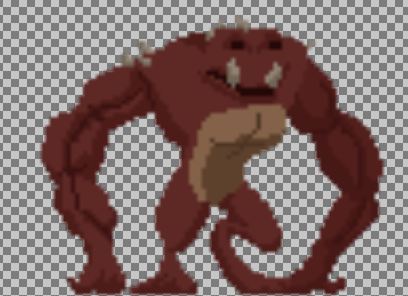
\includegraphics[width=1.0\linewidth]{froggie.png}    
    \caption{
      "Frogman, the King of Deadlift Leverages. The deadlift is performed by picking up the weight from the ground, so this frog has great leverages for the exercise."
    }
    \label{fig:frogman} 
\end{figure}

Users overall seemed to the animated pixel art for the user and the enemies. User 7 mentioned how he enjoyed tracking workouts as he could see the eenmy take damage in a battle "Oh, you know, I get to put in, you know, by my like, 14 sets or whatever I did. And I get to see the boss taking damage." User 4 also mentioned the satisfaction of entering workouts: "I kind of saw it as a sort of a motivation thing, and sort of to get you to train and give you the extra wee bit of dopamine from training and when logging your workout"

Generally, users suggested adding more animations sounds and animations.  User 6 suggested that all inputs should have some kind of satisfying feedback: "If its not visually stimulating it's not going to be interesting, it's like filling out a spreadsheet". User 7 used the term "dopamine factory" to  describe making the app as addiciting as possibe. This would involve animations and sounds, and adding a "lootcrate" system to the game, where users unlock chests containing items, which would all be animated. 


A couple users did not like how I had implemented overflow effects. By default, any damage that brings an enemy below zero health is wasted, and not dealt toward the next enemy. This was easier to implement, and I decided to leave it in to see if this would lead to more collaboration. Users would need to coordinate their workouts amongst themselves to minimize wasted damage.

\subsection{Ethical considerations}
When designing my app, I implemented alerts which are triggered if users progress too quickly to prevent users from progressing without caring about technique. Users raised other potential ethical considerations to my app which I had not accounted for. User 1 mentioned how my app could lead to users doing too many workouts: "If I do like five gym sessions per week, but if that wouldn't be enough [to defeat the enemy], it wouldn't be very good for my health like to do like, seventh or eighth, gym session.". In a similar vain, User 4 thinks that my app could lead to users prioritizing game progress over sensible training if the game is poorly balanced: "You shouldn't be able to game the system, do lots of fluff work just to inflate your numbers, all training styles should be accounted for". User 7 mentioned that I should be considerate about adding new features, such as calorie tracking: "It would probably lead to eating disorders where people lose a bunch of weight".

\subsection{Design ideas}
A common feature suggestion was that exercises should be divided by bodypart. In addition to making searching for exercises a bit easier, users liked and suggested adding this as an in-game feature. "Yeah it makes kind of sense if you have bodypart specific armor that like maybe if you do arms a lot you get a battle axe." I discussed this idea further with users who had some experience with games and RPG's. 

"There should be rewards for using and engaging with the app that don't require real world improvement"
User 5
 "Battle pass like in Fortnite and Warzone, where you have to level up in order to get the next tier, and users could pay to get more rewards"
  "You need to add a lot of content, as muscle building and training can be a slow process"

  User 6
  "First person to reach x level or beat y challenge wins something"
    Could literally be a real life sponsor, such as a supplement company
  "If you kill a certain enemy 10 times you get a weapon"
Different types of characters based on what sport you compete in
Create PVP battles, but also player versus NPC battles, such as against popular athletes

User 8
  "Maybe if you could see, like, like, all the avatars maybe, and like, cover kind of like if you if you improve, whatever. If you improve your strength by this much, you'll get a new avatar or something or something like that."
  One friend who only contributed like one workout had such low damage that he lost interest in playing
    "There was [anonymous user] in our group but he was a beginner so he was barely able to contribute."
      I mentioned that all users should have some kind of initial boost that they should get. He thought this was a good idea as strength would be rewarded but users wouldn't be 10 times stronger.

"But they're like, we need to do 100 trillion damage to him" (global enemy fights)
"But you could make item level a thing. where every item you get will have a higher item level. And maybe that needs to be somehow tied to the amount that you use the app."



\subsection{Collaboration vs competitiveness}
User 7 and User 8 were both in the same teamI asked both users whether their motivation was driven by collaboration or competition. User 7, who was strongest in the team responded: "I think, at the start, I would tell User 8 'Yo, I just did a workout I just did this much damage, the boss is almost dead, you need to work out'". This was mostly collaborative: User 7 trained to help the team out, and wanted the User 8 to help him defeat the enemies. I asked User 8 the same question, and he reiterated the same sentiment as User 7: "We never spoke about being competitive". User 8 was a bit weaker than User 7, and he gave me insight into how this influenced his motivation: "I think User 7 did a couple more workouts than me, and I was trying to keep up with him. I think it was definetely competitive there." This intrigued me, as User 8 felt competive as the underdog, but the strongest member in the team did not feel competitive. This lead to User 8 putting in more effort: "The app probably added an extra workout every week." This is what I hoped that the app design would lead to: users that are weaker and who train less wanting to keep up with other users












    

User 2: tracked lifts, didn't join group and dropped out
  Tracked lifts before "Just have a piece of paper in my kitchen?" Also has training experience
  Import export exercises
  





User 4: Strong, didn't know who they trained with (wanted to find out how the experience was) also didn't drop out. 
  "I was gonna try and get my girlfriend to sign up as well but I don't think she was really able to train consistently"
  "But I still feel is really beneficial. I still feel I got like a good experience from it."
  "I cared more about the workouts because I feel like there was more of a sense of progress with them."
  "But I did think, yeah, I felt like in terms of my character, there wasn't too much progression there. The goal for me was the battles I think." 
  "For me, I didn't really struggle with motivation, right? I would be working out the same whether I had this app or not. I think I like the fact that it was it was a bit of extra reward."

  Question: "I wanted advanced people have to work like a year to add like two kilos. So I kind of wanted to just reward their effort. So as an advanced lifter, would you say that it worked in your case?"
    Answer: "I would say so. Yeah, it's exactly like you said in terms of the character progression"

  Misc
    Used websites which tell you relative strength, such as Symmetric Strength before, which all my calculations are based on. Makes sense why he enjoyed the app
    Liked how simple the app was and how little effort it took to use
    Cardio 
    Uses EFT training app
    He could imagine it being used even in conjuction with other apps (I didn't think anyone would use two apps over the long term.)
    If I branch out and try to be an exercise tracker then I would have more competition

  Issues
    Show how close you are to reaching the next category (if I'm at the top of intermediate I need to push myself a bit more)
    Should be able to track workouts from the past so you don't feel like you're cheating by tracking multiple at once.
    Damage calculations should be more transparent.
    Keyboard blocked the track workouts button

User 5: joined group, invited friend, but didn't really engage with the app, little training experience, has played "Gatcha games" which are essentially super grindy mobile games
 "So the gym has been open and closed and I don't really go to the gym. "
 "If I could've I probably probably would have [used the app] because it would have made actually go to the gym slightly more fun."
  Me: "Do you think them like wanting to progress further or them being stuck on an enemy? Would that on its own be enough for you to actually start training? Just to help them out?"
    Answer: "Probably. Yeah. I do it for that. I do it for like the greater good."
   Game ideas

User 6: used the app briefly but didn't really engage with it, has experience with grindy Gatcha games, also artist
  Split exercises more based on bodyweight and equipment, maybe guide noobies a bit
  Give users sample workouts
  "It was a bit scary and disorienting to start using the app"

User 7: 3 person team, very active, the strongest in that team  
  "Yeah, it wasn't it was quite funny at the start because we were just each of us were just wanting the bosses pretty much at the start but then a lot more. Got more interesting where we can have to work together to kill each boss."
  What about for weight loss

  Issues
    "But it kind of feels a bit frustrating if the boss is 2 health and I've got a workout that has like 40 damage. Like, it's kind of sucks that the damage hasn't gone to the net. I know, it kind of probably shouldn't work that way. I tried splitting my workout into two. So I'd like take like two sets and then kill the boss. So that and then add another workout right after that. I had like 14 if I did like a total of 16. I'm not sure if that's like cheating or not."
    Bodyweight squats broken
    Show other users avatars
    RPG could be more interesting you get items by training which gives you items and resources which you can wear based on your skill level

User 8: also in 3 person team, but was a bit weaker
  This user had a lot of the same comments about the app in general as user 7
  As they lived together, they discussed a lot of their issues together and they seemed to share a lot of the same issues (with regards to technological problems). He also expressed the same kinds of concerns over damage overflow for characters.



  Was your app use more competitive or collaborative
  Was your contribution more altruistic or social obligation 
    "It was more that I wanted to at least do my part, and not let User 7 get all the credit." 
  Which was more important, in-group or out-group competition
    "In-group because I knew who I competed with"


User 9: never tracked a single workout, but very actively updated exercises
  Turns out that this user thought that the "all time bests" screen was where you tracked your workout. This made the user frustrated as this screen wasn't meant to be used often, only when you do better than last time.
    I mentioned that I am planning on adding saved workouts that you can track at the gym as you exercise, and they thought it was a good idea.
  "It wasn't as motivating as it could have been, because I didn't really see what other people were actually doing. I just saw like, okay, we like levelled up or something. Then again, I didn't know who did what. I still felt that I was like fighting alone."
    I asked if she had noticed the chat which had automatic updates and messages from other members, which was especially active in her team. She said she saw the icon but thought it was for tutorials
      "I noticed that in the upper corner. I thought it was general information or something. Yeah, I've already read things beforehand, so I don't need to read them again."
        Maybe chat should be its own upper tab?
    She didn't read the tutorial, so I suggested that there would be integrated tutorials in the app, that could even fit the game theme
      She thought this was better than my initial tutorial

  "For me, it was a bit different, because I've never really marked on my trainings or anything."
  Issues
     Hard to find exercises, I suggested dividing exercises by type and bodypart, thought it was a good idea.


User 10: had exercise experience, didn't really engage with the app
  "So the sort of deal damage feature and how you can like be part of a team and then deal damage to other characters, or others. I don't know if that's something I would personally use. But for me personally, I think that just a feature of building a character, to me, that's a unique selling point of in and of its own." 
  Issues  










Team MVP's (1 person)









\section{Guidance}
\begin{itemize}
    \item
        Ask specific questions that address the general problem.
    \item
        Answer them with precise evidence (graphs, numbers, statistical
        analysis, qualitative analysis).
    \item
        Be fair and be scientific.
    \item
        The key thing is to show that you know how to evaluate your work, not
        that your work is the most amazing product ever.
\end{itemize}

\section{Evidence}
Make sure you present your evidence well. Use appropriate visualisations, reporting techniques and statistical analysis, as appropriate.

If you visualise, follow the basic rules, as illustrated in Figure \ref{fig:boxplot}:
\begin{itemize}
\item Label everything correctly (axis, title, units).
\item Caption thoroughly.
\item Reference in text.
\item \textbf{Include appropriate display of uncertainty (e.g. error bars, Box plot)}
\item Minimize clutter.
\end{itemize}

See the file \texttt{guide\_to\_visualising.pdf} for further information and guidance.



%==================================================================================================================================
\chapter{Conclusion}    
Summarise the whole project for a lazy reader who didn't read the rest (e.g. a prize-awarding committee).
\section{Guidance}
\begin{itemize}
    \item
        Summarise briefly and fairly.
    \item
        You should be addressing the general problem you introduced in the
        Introduction.        
    \item
        Include summary of concrete results (``the new compiler ran 2x
        faster'')
    \item
        Indicate what future work could be done, but remember: \textbf{you
        won't get credit for things you haven't done}.
\end{itemize}

%==================================================================================================================================
%
% 
%==================================================================================================================================
%  APPENDICES  

\begin{appendices}



\begin{itemize}
\item
  Copies of ethics approvals (required if obtained)
\item
  Copies of questionnaires etc. used to gather data from subjects.
\item
  Extensive tables or figures that are too bulky to fit in the main body of
  the report, particularly ones that are repetitive and summarised in the body.

\item Outline of the source code (e.g. directory structure), or other architecture documentation like class diagrams.

\item User manuals, and any guides to starting/running the software.

\end{itemize}

\textbf{Don't include your source code in the appendices}. It will be
submitted separately.

\end{appendices}

%==================================================================================================================================
%   BIBLIOGRAPHY   

% The bibliography style is abbrvnat
% The bibliography always appears last, after the appendices.

\bibliographystyle{abbrvnat}

\bibliography{l4proj}



\end{document}

%pemipa5283@990ys.com 
%hatob51724@grokleft.com

User 1: Team MVP and 5 person team member, most active member in the game
  Team MVP
    As he we was annoyed that other users didn't feel an obligation to help, we discussed whether it would make sense to divide users into classes which all have to work together.   When asked how he would feel if they had to rely on their teammates more and someone would still be a broken link, he replied: 
  Most active member  
    "the gyms haven't been even closed, and there's like no restrictions."
    Already trained consistently
    Used fitnotes app before
    Knew the team's members

  Issues
    Exercises unsaving when saving new lifts
    Animations taking a long time to load (probably has to do with calculate strength)
    Thought animations were too pixelated (which is expected for pixel art)
    With regards to user animations
    Add exercise diary, should be game and standalone fitness tracker

User 3: MVP, trained with random users, very strong/experienced
  "Timing was kind of bad because nobody I know was working out during the three weeks I had to actually test it. Even French in other countries, they were in countries that are currently locked down. So they couldn't go to the gym. I'm still working out. But that's because I do bodyweight stuff, so I can do it"


  But simultaneously doesn't think it would be fun to train with someone putting in crazy amounts of work:
  "And then we had one guy who was working out seven out of seven times a week for three to four hours a day. And so imagine that we had that guy in our team: he would be doing like 90\% out of a team of 10 people."

  Misc: 
    Can gym with friends in different locations
    "But no, for two reasons, hey, you're very unlikely to find people that work out and play D\&D"

  Issues:
    Exercise recommendations
    Cardio
    Challenges outside of your skill domain
    Monthly challenges
